\documentclass[12pt,a4paper,oneside]{report}
\usepackage[T1]{fontenc}
\usepackage[utf8]{inputenc}
\DeclareUnicodeCharacter{1D49}{\textsuperscript{e}}
\usepackage[french]{babel}
\usepackage{times}
\usepackage{microtype}
\usepackage{geometry}
\geometry{left=2.5cm,right=2.5cm,top=2.5cm,bottom=2.5cm}
\usepackage{setspace}
\onehalfspacing

% Packages graphiques et couleurs
\usepackage{graphicx}
\usepackage{xcolor}
\usepackage{tikz}
\usepackage{float}

% Couleurs institutionnelles (nécessaires pour titlepage.tex)
\definecolor{ucbBlue}{RGB}{12, 53, 106}
\definecolor{ucbGold}{RGB}{212, 160, 23}
\definecolor{darkGray}{RGB}{60, 60, 60}

\usepackage{booktabs,longtable,array}
\usepackage{calc}
\usepackage{amsmath,amssymb}
\usepackage{enumitem}

\usepackage{csquotes}
\usepackage[backend=biber,style=ieee,sorting=none]{biblatex}
\addbibresource{references.bib}

\usepackage{titlesec}
\usepackage{fancyhdr}

% Hyperref et sous-packages associés
\usepackage{hyperref}
\hypersetup{hidelinks}
\usepackage{url}
\usepackage{caption}

% Configuration des titres et en-têtes
\titleformat{\chapter}[display]{\normalfont\bfseries\centering}{CHAPITRE \Roman{chapter}}{0.5em}{\Large}
\titlespacing*{\chapter}{0pt}{0pt}{1.5em}
\pagestyle{fancy}
\fancyhf{}
\fancyhead[R]{\thepage}
\setlength{\headheight}{14.5pt}
\setcounter{secnumdepth}{3}
\setcounter{tocdepth}{3}

\begin{document}
	
	% 1. Page de garde
%	\begin{titlepage}
    \centering
    
    % En-tête institutionnel
    {{\MakeUppercase{République Démocratique du Congo}}}\\[0.1cm]
    {{\MakeUppercase{Ministère de l'Enseignement Supérieur et Universitaire}}}\\[0.1cm]
    {{\MakeUppercase{Université Catholique de Bukavu}}}\\[1.0cm]
    
    % Logo UCB situé dans le dossier figures
    
\includegraphics[width=3.8cm]{figures/logoucb}\\[0.4cm]

    {\MakeUppercase{UCB}}\\[0.15cm]
    {{FACULTÉ DES SCIENCES}}\\[0.1cm]
    {{\MakeUppercase{Département Système Informatique}}}\\[0.5cm]

    % ::::::::::::::::::::::::::::::::::::::::::::::::::::::
    \rule{\linewidth}{1.2pt}\\[0.2cm]
    {Conception et Développement d’un jumeau numérique intégrant l’intelligence artificielle pour l’optimisation du réseau de fourniture d’eau potable dans la commune de Kadutu}
    \rule{\linewidth}{1.2pt}\\[0.2cm]

    % Nature du document / Type de travail
    {\large \small Projet tutoré}\\[0.1cm]
    {\large \small Présenté pour l'obtention du diplôme de Bacaloreat en Informatiques}\\[1.0cm]
    
    % \vfill




    % Auteur et Encadreurs

    {Présenté par :}\\
    { LANDRY MULUMEODERHWA Landry}
    

    \vfill

    {\large \textbf{Année Académique 2025 - 2026}}

\end{titlepage}
	
	% 2. Table des matières avec numérotation romaine préalable
	\cleardoublepage
	\pagenumbering{roman}
	\pdfbookmark[1]{Table des matières}{toc}
	\tableofcontents
	\newpage
	
	% 3. Corps du document (Numérotation arabe)
	\cleardoublepage
	%% ============================================================
% ÉPIGRAPHE
% ============================================================
\cleardoublepage

\begin{center}
	{\Large \textbf{EPIGRAPHE}}
\end{center}

\vspace*{4cm}

\begin{flushright}
	\textit{%
		« La technologie ne remplace pas l'intelligence humaine ;\\
		elle lui donne les moyens d'aller plus loin. »
	}
	
	\vspace{0.5cm}
	
	--- Stephen Hawking
\end{flushright}

\cleardoublepage
	%% ============================================================
% DÉDICACE
% ============================================================
\cleardoublepage

\begin{center}
	{\Large \textbf{DÉDICACE}}
\end{center}

\vspace{2cm}

\begin{flushleft}
	
	À Dieu Tout-Puissant, source de vie, de sagesse et de
	persévérance, pour m'avoir accompagné tout au long de mon
	parcours académique.
	
	\vspace{0.5cm}
	
	À mes parents, pour leurs sacrifices, leur amour, leurs
	encouragements et leur soutien inconditionnel.
	
	\vspace{0.5cm}
	
	À ma famille, pour sa présence, ses conseils et son affection.
	
	\vspace{0.5cm}
	
	À mes enseignants et encadreurs, pour les connaissances,
	les orientations et les conseils qui ont contribué à ma
	formation.
	
	\vspace{0.5cm}
	
	À toutes les personnes qui, de près ou de loin, ont contribué
	à la réalisation de ce travail, je dédie ce mémoire avec
	profonde reconnaissance.
	
	\vspace{1cm}
	
	\begin{center}
		\textbf{À vous tous, je dédie ce travail.}
	\end{center}
	
\end{flushleft}

\cleardoublepage
	%% ============================================================
% RÉSUMÉ
% ============================================================
\cleardoublepage
\chapter*{RÉSUMÉ}
\addcontentsline{toc}{chapter}{Résumé}

L'approvisionnement en eau potable constitue un enjeu majeur
pour les populations urbaines, particulièrement dans les zones
où les réseaux de distribution sont confrontés à des problèmes
de pertes d'eau, de variations de pression, de défaillances des
équipements et de difficultés de surveillance. Dans la commune
de Kadutu, à Bukavu, ces contraintes rendent nécessaire la mise
en place de solutions technologiques capables d'améliorer la
gestion et le suivi du réseau.

Le présent travail porte sur le \textbf{développement d'un
	jumeau digital intégrant l'intelligence artificielle pour
	l'optimisation du réseau de fourniture d'eau potable dans la
	commune de Kadutu}. L'objectif est de concevoir une représentation
numérique du réseau permettant de suivre son fonctionnement,
de simuler différents scénarios et d'identifier plus rapidement
certaines anomalies susceptibles d'affecter la distribution
de l'eau.

La solution proposée s'appuie sur une architecture informatique
intégrant une base de données, une interface de visualisation
géographique, une API développée avec \textbf{FastAPI}, ainsi
que des techniques d'intelligence artificielle destinées à
l'analyse des données du réseau. Le système permet notamment
de représenter les principaux éléments du réseau, de surveiller
certains paramètres, de simuler des situations de dysfonctionnement
et de faciliter la prise de décision.

Les résultats attendus montrent qu'un jumeau digital associé
à l'intelligence artificielle peut constituer un outil d'aide
à la gestion, à la surveillance et à la maintenance du réseau
d'eau potable. Une telle approche contribue à améliorer la
connaissance du réseau, à anticiper certaines anomalies et à
soutenir une gestion plus efficace des ressources en eau.

\vspace{0.5cm}

\noindent\textbf{Mots-clés :} Jumeau digital, intelligence
artificielle, réseau d'eau potable, optimisation, détection
d'anomalies, simulation, FastAPI, Kadutu.

\cleardoublepage
	
	% DEBUT DU CHIFRE ARABE
	\pagenumbering{arabic}
	
	\chapter*{INTRODUCTION}\addcontentsline{toc}{chapter}{INTRODUCTION}\label{introduction}

\section{CONTEXTE GÉNÉRAL DE L'ÉTUDE}
\label{contexte-general-de-letude}

L'accès à une eau potable sûre et disponible de manière régulière demeure
un enjeu important dans de nombreux pays en développement. Selon le
Programme commun de suivi de l'Organisation mondiale de la Santé (OMS)
et du Fonds des Nations Unies pour l'enfance (UNICEF), près de
2,2 milliards de personnes ne disposaient pas, en 2022, d'un service
d'eau potable géré en toute sécurité \cite{ref1}. Cette situation montre
que l'amélioration de l'accès à l'eau potable ne dépend pas uniquement
de la disponibilité de la ressource, mais également de la capacité à
assurer une gestion efficace et durable des infrastructures de
distribution.

En République Démocratique du Congo, cette problématique demeure
particulièrement importante dans les centres urbains où l'augmentation
de la population et l'extension des zones d'habitation exercent une
pression croissante sur les infrastructures existantes. Dans ce
contexte, la continuité de la desserte dépend notamment de l'état des
conduites, du fonctionnement des équipements hydrauliques, de la
disponibilité de l'eau et de la capacité des services techniques à
identifier et à traiter rapidement les anomalies. Les difficultés de
surveillance et de maintenance peuvent ainsi se traduire par des
interruptions de service, des pertes d'eau et des interventions
principalement effectuées après l'apparition d'une défaillance.

La ville de Bukavu présente ces enjeux dans un contexte urbain
particulier, caractérisé par une forte densité de population et une
extension progressive des zones d'habitation. La commune de Kadutu,
qui constitue l'une des communes de la ville, est directement concernée
par ces difficultés. Les observations réalisées au cours de la phase
exploratoire de cette étude, associées aux informations disponibles
dans les sources documentaires, montrent notamment l'existence de
perturbations de la desserte en eau potable dans certains secteurs de
Kadutu. En juillet 2022, l'Agence Congolaise de Presse rapportait par
exemple que certaines avenues de la commune rencontraient des
difficultés d'approvisionnement en eau distribuée par la REGIDESO,
avec une situation particulièrement préoccupante durant la saison
sèche \cite{ref127}.

Dans ce contexte, la gestion efficace du réseau de fourniture d'eau
potable de Kadutu nécessite non seulement des infrastructures physiques
adaptées, mais également des moyens permettant de mieux connaître
l'état du réseau et de suivre son fonctionnement. Or, les informations
relatives aux différents éléments du réseau, à leur état, à leur
localisation et à leur fonctionnement ne sont pas toujours regroupées
dans un environnement numérique permettant une exploitation et une
analyse centralisées. Cette situation rend plus difficile la
visualisation globale du réseau et l'identification rapide des secteurs
susceptibles de nécessiter une intervention.

Les progrès récents de l'intelligence artificielle et des technologies
de représentation numérique offrent cependant de nouvelles possibilités
pour répondre à ce type de difficulté. Le jumeau numérique permet de
représenter virtuellement un système physique et de faire évoluer cette
représentation à partir des données disponibles. Associé à des
techniques d'intelligence artificielle, il peut être utilisé pour
analyser les données du réseau, identifier certaines anomalies et
simuler des situations de fonctionnement. De telles possibilités sont
particulièrement intéressantes dans le contexte de Kadutu, où
l'amélioration de la connaissance du réseau et de sa surveillance peut
constituer un appui à la maintenance et à la prise de décision
\cite{ref9}.

C'est donc dans le contexte spécifique du réseau de fourniture d'eau
potable de la commune de Kadutu que s'inscrit la présente étude. Elle
vise à étudier la possibilité de mettre en place un jumeau numérique
intégrant des techniques d'intelligence artificielle afin de disposer
d'une représentation numérique du réseau, de faciliter sa surveillance,
d'identifier certaines anomalies et de fournir un support à la
planification des interventions de maintenance.


\section{PROBLÉMATIQUE}
\label{problematique}

Dans la commune de Kadutu, la gestion du réseau de fourniture d'eau
potable est confrontée à plusieurs difficultés qui limitent la capacité
à assurer un suivi efficace de son fonctionnement. Les perturbations
observées dans la desserte constituent l'un des principaux problèmes.
Certaines zones peuvent connaître des interruptions ou une distribution
irrégulière de l'eau, notamment dans certaines périodes de l'année.
Ces situations nécessitent de pouvoir déterminer rapidement les parties
du réseau concernées et d'identifier les facteurs susceptibles
d'expliquer la perturbation.

Un second problème concerne la connaissance et la surveillance du
réseau. Un réseau de fourniture d'eau est constitué de plusieurs
éléments interdépendants, notamment des conduites, des nœuds, des
réservoirs, des vannes et des points de desserte. Lorsque les
informations relatives à ces éléments ne sont pas représentées dans un
environnement numérique centralisé et facilement exploitable, il
devient plus difficile d'obtenir une vision globale de la structure du
réseau et de suivre son évolution. Cette insuffisance peut compliquer
l'analyse d'une anomalie et la localisation de la zone nécessitant une
intervention.

À cette difficulté s'ajoute la détection des anomalies pouvant affecter
le fonctionnement du réseau. Une baisse anormale de pression, une
variation inhabituelle du débit, une rupture de conduite ou une fuite
peuvent perturber la desserte et entraîner des pertes d'eau. Lorsque
ces phénomènes ne sont pas détectés suffisamment tôt, leur localisation
et leur prise en charge peuvent devenir plus difficiles. La disponibilité
de données structurées et leur analyse automatique pourraient donc
permettre d'améliorer la détection des situations anormales.

La maintenance constitue également un enjeu important. En l'absence
d'un outil permettant de centraliser les informations sur le réseau et
d'analyser son état, les interventions peuvent être davantage orientées
vers la réaction à une panne déjà apparue que vers son anticipation.
Cette situation limite la possibilité de hiérarchiser les zones
nécessitant une attention particulière et de préparer les interventions
sur la base d'informations relatives au fonctionnement du réseau.

Ainsi, le problème central identifié dans le cadre de cette étude n'est
pas uniquement l'existence de perturbations dans la fourniture d'eau,
mais également la difficulté à disposer d'un outil numérique permettant
de représenter le réseau de Kadutu, de suivre son fonctionnement,
d'identifier les anomalies et d'appuyer les décisions de maintenance.
L'insuffisance d'une telle représentation dynamique constitue une limite
pour une gestion fondée sur les données.

Le projet de jumeau numérique proposé dans cette étude cherche donc à
répondre à ces insuffisances en développant une représentation
numérique du réseau de fourniture d'eau potable de Kadutu. L'intégration
de techniques d'intelligence artificielle doit permettre d'exploiter les
données disponibles afin de contribuer à la détection des anomalies et
à l'analyse du fonctionnement du réseau. Le système envisagé doit
également permettre de visualiser les différents composants du réseau,
de simuler certaines situations et de fournir des informations utiles
à l'identification des secteurs nécessitant une intervention.

Dès lors, la question fondamentale qui guide cette étude est la
suivante :

\textbf{Comment la conception et le développement d'un jumeau numérique
	intégrant des techniques d'intelligence artificielle peuvent-ils
	contribuer à améliorer la surveillance, la détection des anomalies et
	la maintenance du réseau de fourniture d'eau potable de la commune de
	Kadutu ?}

\section{HYPOTHÈSES DE RECHERCHE}
\label{hypotheses-de-recherche}

\subsection{Hypothèse générale}
\label{hypothese-generale}

La mise en œuvre d'un \textbf{jumeau numérique intégrant des techniques
	d'intelligence artificielle} devrait améliorer la surveillance du
réseau de fourniture d'eau potable de la commune de \textbf{Kadutu},
faciliter la détection des anomalies et contribuer à une maintenance
plus efficace grâce à l'exploitation des données du réseau.

\subsection{Hypothèses spécifiques}
\label{hypotheses-specifiques}

Afin de répondre à la problématique de recherche, les hypothèses
spécifiques suivantes sont formulées :

\subsection{Première hypothèse spécifique}
\label{premiere-hypothese-specifique}

La modélisation numérique du réseau de fourniture d'eau potable de
\textbf{Kadutu} permettrait d'améliorer sa représentation, sa
visualisation et le suivi de ses différents composants.

\subsection{Deuxième hypothèse spécifique}
\label{deuxieme-hypothese-specifique}

L'intégration des données relatives au fonctionnement du réseau
permettrait d'améliorer la surveillance de celui-ci et de faciliter
l'identification des variations anormales de ses paramètres.

\subsection{Troisième hypothèse spécifique}
\label{troisieme-hypothese-specifique}

L'utilisation de techniques d'\textbf{intelligence artificielle}
permettrait de détecter automatiquement certaines anomalies du réseau
et de contribuer à l'anticipation des défaillances.

\subsection{Quatrième hypothèse spécifique}
\label{quatrieme-hypothese-specifique}

L'intégration du jumeau numérique et de l'intelligence artificielle
pourrait fournir aux gestionnaires des informations utiles à la
planification et à la priorisation des interventions de maintenance.

\section{OBJECTIFS DE L'ÉTUDE}
\label{objectifs-de-letude}

\subsection{Objectif général}
\label{objectif-general}

L'objectif général de cette étude est de \textbf{concevoir et développer
	un jumeau numérique intégrant des techniques d'intelligence artificielle}
pour améliorer la surveillance, la détection des anomalies et la
maintenance du réseau de fourniture d'eau potable de la commune de
Kadutu.

\subsection{Objectifs spécifiques}
\label{objectifs-specifiques}

\noindent{Pour atteindre cet objectif général, la présente étude vise à :}

\noindent\textbf{Analyser le réseau de fourniture d'eau potable de la
	commune de Kadutu} afin d'identifier ses principales composantes, son
fonctionnement et les difficultés liées à sa surveillance et à sa
maintenance ;

\noindent\textbf{Modéliser numériquement le réseau de fourniture d'eau
	potable de la commune de Kadutu} en représentant ses principaux
composants et leurs relations ;

\noindent\textbf{Mettre en place un mécanisme de collecte et
	d'intégration des données du réseau} afin de faciliter le suivi de son
état et de ses paramètres de fonctionnement ;

\noindent\textbf{Intégrer des techniques d'intelligence artificielle}
pour analyser les données du réseau et détecter certaines anomalies
susceptibles d'affecter son fonctionnement ;

\noindent\textbf{Développer une plateforme de jumeau numérique}
permettant de visualiser le réseau de la commune de Kadutu, de suivre
son état, de simuler certaines situations et de fournir des
informations utiles à la planification des interventions de
maintenance.

\section{INTÉRÊT DE
L\textquotesingle ÉTUDE}\label{intuxe9ruxeat-de-luxe9tude}

\subsection{Intérêt
scientifique}\label{intuxe9ruxeat-scientifique}

Sur le plan scientifique, cette étude contribue à enrichir les travaux
portant sur l\textquotesingle application des technologies du
\textbf{jumeau numérique}, de l\textquotesingle Internet des objets et
de l\textquotesingle intelligence artificielle dans le domaine de la
gestion des réseaux de distribution d\textquotesingle eau potable. Elle
participe également à l\textquotesingle adaptation de ces technologies
au contexte des pays en développement, et plus particulièrement à celui
de la République Démocratique du Congo, où peu de recherches ont
jusqu\textquotesingle à présent porté sur leur mise en œuvre dans les
infrastructures hydrauliques urbaines.

\subsection{Intérêt pratique}\label{intuxe9ruxeat-pratique}

Sur le plan pratique, cette étude vise à proposer une solution
susceptible d\textquotesingle améliorer la surveillance, la maintenance
et la planification du réseau de fourniture d\textquotesingle eau
potable de la commune de Kadutu. Les résultats attendus pourront servir
d\textquotesingle outil d\textquotesingle aide à la décision pour la
REGIDESO et les autorités compétentes, en facilitant la détection des
anomalies, la réduction des pertes d\textquotesingle eau,
l\textquotesingle optimisation des interventions techniques et
l\textquotesingle amélioration de la qualité du service rendu aux
usagers.

\section{DÉLIMITATION DE L'ÉTUDE}
\label{delimitation-de-letude}

\subsection{Délimitation spatiale}
\label{delimitation-spatiale}

La présente étude est réalisée dans la \textbf{commune de Kadutu},
située dans la ville de Bukavu, province du Sud-Kivu, en République
Démocratique du Congo. Elle porte spécifiquement sur le réseau de
fourniture d'eau potable de cette commune et vise à y expérimenter une
approche basée sur le jumeau numérique.

\subsection{Délimitation temporelle}
\label{delimitation-temporelle}

Cette recherche couvre la période allant de \textbf{2025 à 2026},
correspondant aux différentes étapes de l'étude, notamment la collecte
et l'analyse des données relatives à la structure, à la localisation et
aux caractéristiques techniques du réseau de fourniture d'eau potable
de la commune de Kadutu, ainsi qu'à la conception, au développement et à
l'évaluation du jumeau numérique proposé.

\subsection{Délimitation thématique}
\label{delimitation-thematique}

La présente étude s'inscrit dans le domaine de l'informatique appliquée,
plus précisément dans les thématiques du \textbf{jumeau numérique} et
de l'\textbf{intelligence artificielle} appliqués à la surveillance,
à la détection des anomalies et à la maintenance du réseau de
fourniture d'eau potable de la commune de Kadutu.

\subsection{Délimitation méthodologique}
\label{delimitation-methodologique}

Sur le plan méthodologique, l'étude porte sur l'analyse du réseau
existant, la collecte et la structuration des données disponibles, la
modélisation numérique de ses principaux composants, puis la conception
et le développement d'un prototype de jumeau numérique intégrant des
techniques d'intelligence artificielle. L'évaluation porte sur les
fonctionnalités de représentation du réseau, de surveillance, de
simulation et de détection des anomalies. Les résultats obtenus sont
évalués dans le cadre du prototype développé et ne prétendent pas
constituer une généralisation à l'ensemble des réseaux de fourniture
d'eau potable de la ville de Bukavu.

\section{SUBDIVISION DU MÉMOIRE}\label{subdivision-du-muxe9moire}

Le présent mémoire est subdivisé en \textbf{quatre chapitres} :

\begin{itemize}
\item
  \textbf{Chapitre I :} Revue de la littérature et fondements
  théoriques.
\item 
  \textbf{Chapitre II :} Matériels et méthodes.
\item
  \textbf{Chapitre III :} Conception et développement du jumeau
  numérique intégrant l\textquotesingle intelligence artificielle.
\item
  \textbf{Chapitre IV :} Présentation, analyse et discussion des
  résultats.
\end{itemize}

\clearpage
% ------- Fin de l'introduction
	```latex
\chapter{REVUE DE LA LITTÉRATURE ET FONDEMENTS THÉORIQUES}
\label{chapitre-i-revue-de-la-litterature-et-fondements-theoriques}

\section{Concepts fondamentaux liés à la distribution de l'eau potable}
\label{concepts-fondamentaux-lies-a-la-distribution-de-leau-potable}

\subsection{Définition de l'eau potable}
\label{definition-de-leau-potable}

L'eau potable désigne une eau dont les caractéristiques physiques,
chimiques, biologiques et microbiologiques respectent les exigences
nécessaires à la consommation humaine sans risque significatif pour la
santé. Sa sécurité doit être maintenue tout au long de la chaîne
d'approvisionnement, depuis le captage jusqu'au consommateur
\cite{ref4}, \cite{ref23}.

L'accès à une eau potable sûre constitue également un droit humain
fondamental reconnu par les Nations Unies et participe à la réalisation
de l'Objectif de développement durable 6 (ODD 6), consacré à l'eau
potable et à l'assainissement \cite{ref3}. Dans cette perspective, la
qualité de l'eau dépend non seulement du traitement, mais également de
la fiabilité des infrastructures chargées de son transport et de sa
distribution \cite{ref1}.

\subsection{Réseau de distribution d'eau potable}
\label{reseau-de-distribution-deau-potable}

Le réseau de distribution d'eau potable est l'ensemble des ouvrages et
équipements permettant d'acheminer l'eau traitée jusqu'aux points de
consommation. Il comprend notamment les conduites, les réservoirs, les
stations de pompage, les vannes, les dispositifs de contrôle et les
équipements de mesure \cite{ref11}.

Le fonctionnement du réseau dépend de l'interaction entre ces différents
éléments. Une défaillance d'une conduite, d'une pompe, d'une vanne ou
d'un réservoir peut entraîner une baisse de pression, une interruption
de service ou une perte d'eau. La surveillance de paramètres tels que
la pression, le débit et le niveau des réservoirs constitue donc une
condition importante pour assurer la continuité du service \cite{ref20}.

\subsection{Composantes du réseau}
\label{composantes-du-reseau}

Les principales composantes d'un réseau d'alimentation en eau potable
sont les ouvrages de captage, les stations de traitement, les réservoirs,
les conduites, les stations de pompage et les vannes. Les conduites
assurent le transport de l'eau, les réservoirs permettent son stockage et
la régulation du système, tandis que les pompes et les vannes contribuent
au maintien des conditions hydrauliques nécessaires à la distribution
\cite{ref33}, \cite{ref34}, \cite{ref35}.

Dans les réseaux modernes, des capteurs peuvent être associés à ces
composants afin de mesurer différents paramètres de fonctionnement.
Ces informations constituent une base importante pour la surveillance
numérique et l'analyse de l'état du réseau \cite{ref20}.

\section{Déploiement d'un réseau de distribution d'eau potable}
\label{deploiement-dun-reseau-de-distribution-deau-potable}

Le déploiement d'un réseau d'eau potable comprend la planification, la
conception, le dimensionnement et l'installation des infrastructures
nécessaires à la desserte d'une population. Il doit tenir compte des
besoins en eau, de la topographie, de la répartition de la population,
des capacités des infrastructures existantes et des possibilités
d'extension du réseau \cite{ref38}, \cite{ref39}.

La planification spatiale permet de déterminer la localisation des
conduites, des réservoirs et des équipements hydrauliques. Les systèmes
d'information géographique (SIG) peuvent faciliter cette représentation
et l'identification des zones insuffisamment desservies. De même, la
modélisation hydraulique, notamment avec des outils tels qu'EPANET,
permet d'étudier les pressions, les débits et différents scénarios de
fonctionnement avant la réalisation des infrastructures
\cite{ref40}, \cite{ref34}.

Dans le cadre de cette étude, le déploiement est considéré comme une
dimension complémentaire de la gestion du réseau de la commune de
Kadutu, notamment pour la représentation spatiale et la simulation de
scénarios d'évolution du réseau.

\section{Surveillance d'un réseau de distribution d'eau potable}
\label{surveillance-dun-reseau-de-distribution-deau-potable}

La surveillance consiste à suivre l'état des infrastructures et
l'évolution des principaux paramètres hydrauliques du réseau. Elle vise
notamment à détecter les fuites, les ruptures, les baisses de pression
et les dysfonctionnements des équipements \cite{ref11}.

Les méthodes traditionnelles reposent principalement sur les inspections
de terrain, les relevés manuels et les signalements des usagers. Elles
peuvent toutefois présenter des limites lorsqu'une anomalie survient
entre deux inspections ou lorsqu'une fuite reste difficilement visible
\cite{ref45}.

L'utilisation de capteurs, de SIG et de plateformes numériques permet
d'améliorer la collecte, la visualisation et l'analyse des informations
relatives au réseau. L'objectif est progressivement de passer d'une
surveillance essentiellement réactive à une surveillance davantage
proactive et fondée sur les données \cite{ref20}, \cite{ref47}.

Dans le présent travail, la surveillance constitue l'une des fonctions
principales du jumeau numérique du réseau de fourniture d'eau potable de
la commune de Kadutu.

\section{Maintenance d'un réseau de distribution d'eau potable}
\label{maintenance-dun-reseau-de-distribution-deau-potable}

La maintenance regroupe les actions visant à maintenir ou à rétablir les
infrastructures dans un état permettant d'assurer la continuité et la
fiabilité du service. Elle peut être corrective, préventive ou
prédictive \cite{ref42}.

La maintenance corrective intervient après une panne, tandis que la
maintenance préventive repose sur des opérations planifiées. La
maintenance prédictive cherche, quant à elle, à exploiter les données
disponibles afin d'identifier les signes annonciateurs d'une défaillance
et de faciliter la planification des interventions \cite{ref45},
\cite{ref49}, \cite{ref47}.

Les fuites constituent un problème important des réseaux d'eau potable.
La surveillance de la pression et du débit, associée à l'analyse des
données, peut contribuer à détecter plus rapidement certaines situations
anormales \cite{ref50}, \cite{ref20}. Dans cette étude, la maintenance
est principalement envisagée sous l'angle de l'aide à la détection des
anomalies et de la priorisation des interventions.

\section{Technologies numériques appliquées à la gestion des réseaux d'eau potable}
\label{technologies-numeriques-appliquees-a-la-gestion-des-reseaux-deau-potable}

La transformation numérique des réseaux d'eau repose sur plusieurs
technologies complémentaires. Les SIG permettent de représenter
spatialement les infrastructures, tandis que l'Internet des objets (IoT)
et les capteurs facilitent la collecte des données de fonctionnement
\cite{ref52}, \cite{ref20}.

Les systèmes de supervision, les bases de données et les solutions
informatiques permettent ensuite de centraliser et d'exploiter les
informations collectées. Les systèmes SCADA sont principalement orientés
vers la supervision et le contrôle, alors que le jumeau numérique ajoute
une dimension de représentation virtuelle, de simulation et d'analyse
\cite{ref54}.

L'intelligence artificielle complète cette chaîne technologique en
permettant l'analyse des données, la détection des anomalies et la
production de prédictions. L'intérêt de ces technologies réside surtout
dans leur intégration au sein d'une architecture cohérente
\cite{ref55}, \cite{ref56}.

\section{Le concept de jumeau numérique (Digital Twin)}
\label{le-concept-de-jumeau-numerique-digital-twin}

Un jumeau numérique est une représentation numérique dynamique d'un
système physique, maintenue en relation avec celui-ci par l'échange de
données. Contrairement à une simple maquette ou à un modèle statique, il
est capable d'évoluer en fonction de l'état observé du système réel
\cite{ref8}, \cite{ref58}.

Le concept est notamment associé aux travaux de Michael Grieves dans le
domaine de la gestion du cycle de vie des produits. Son évolution a été
favorisée par le développement des capteurs, de l'IoT, des bases de
données, de l'informatique en nuage et de l'intelligence artificielle
\cite{ref59}.

Un jumeau numérique repose généralement sur trois éléments essentiels :
le système physique, sa représentation virtuelle et le mécanisme
d'échange de données. Cette organisation permet d'observer l'état du
système, d'analyser son fonctionnement et de simuler différents
scénarios \cite{ref60}.

Dans le domaine de l'eau potable, un jumeau numérique peut représenter
les conduites, les réservoirs, les pompes, les vannes et les autres
composants du réseau. Il peut également intégrer des données de pression,
de débit et de niveau afin de suivre l'état du système et de faciliter
l'analyse des anomalies \cite{ref20}.

Dans le cadre de cette étude, le jumeau numérique est défini comme une
\textbf{représentation virtuelle dynamique du réseau de fourniture d'eau
	potable de la commune de Kadutu}. Il a pour rôle de faciliter la
visualisation du réseau, le suivi de son état, la simulation de certaines
situations et l'aide à la détection des anomalies.

\section{Architecture et fonctionnement d'un jumeau numérique}
\label{architecture-et-fonctionnement-dun-jumeau-numerique}

L'architecture d'un jumeau numérique assure la circulation des données
entre le système physique et sa représentation virtuelle. Elle comprend
généralement une couche physique, des dispositifs de collecte, une
couche de communication, une base de données, un modèle numérique, une
couche d'analyse et une interface de visualisation \cite{ref60}.

Dans un réseau d'eau potable, les capteurs peuvent fournir des mesures
de pression, de débit ou de niveau. Ces données sont transmises,
stockées puis analysées avant d'être présentées sur une interface
permettant aux gestionnaires de suivre l'état du réseau. L'intelligence
artificielle peut être intégrée à cette architecture afin de renforcer
la détection des anomalies et l'aide à la maintenance \cite{ref61}.

Dans cette étude, cette architecture est adaptée au réseau de fourniture
d'eau potable de la commune de Kadutu et sert de base au prototype
développé dans le chapitre III \cite{ref65}.

\section{Intelligence artificielle appliquée à la gestion des réseaux d'eau potable}
\label{intelligence-artificielle-appliquee-a-la-gestion-des-reseaux-deau-potable}

L'intelligence artificielle regroupe des méthodes permettant à un système
informatique d'exploiter des données afin d'effectuer des tâches
d'analyse, de classification ou de prédiction. Parmi ses principales
branches figure l'apprentissage automatique (\emph{Machine Learning}),
qui permet à un modèle d'apprendre des relations à partir de données
\cite{ref67}, \cite{ref69}.

L'apprentissage automatique comprend notamment l'apprentissage supervisé,
non supervisé et par renforcement. Pour la gestion des réseaux d'eau,
plusieurs algorithmes peuvent être utilisés, tels que les arbres de
décision, les forêts aléatoires, les SVM et les réseaux de neurones,
selon la nature des données et le problème étudié \cite{ref70},
\cite{ref71}.

L'intelligence artificielle peut notamment être utilisée pour détecter
des anomalies, identifier des comportements inhabituels, analyser les
variations de pression et de débit et contribuer à l'anticipation de
certaines défaillances \cite{ref73}.

Dans le présent travail, l'IA est intégrée au jumeau numérique pour
analyser les données disponibles et contribuer à la détection de
certaines anomalies du réseau de la commune de Kadutu. Son utilisation
reste un outil d'aide à la décision et ne se substitue pas à
l'expertise des gestionnaires.

\section{Intégration du jumeau numérique et de l'intelligence artificielle}
\label{integration-du-jumeau-numerique-et-de-lintelligence-artificielle}

Le jumeau numérique fournit une représentation dynamique du système
physique, tandis que l'intelligence artificielle apporte des capacités
d'analyse et de détection. Leur intégration permet donc de transformer
une simple représentation numérique en un système capable d'exploiter les
données pour améliorer la surveillance et la maintenance
\cite{ref60}, \cite{ref61}.

Dans un réseau d'eau potable, les données relatives à la pression, au
débit ou à d'autres paramètres peuvent être analysées afin d'identifier
des comportements inhabituels. Les résultats peuvent ensuite être
présentés sous forme d'alertes ou d'informations utiles à la
priorisation des interventions.

Cette intégration présente toutefois des limites, notamment la
disponibilité des données, leur qualité, l'interopérabilité des
technologies et les contraintes liées aux ressources techniques et
financières \cite{ref60}. Ces contraintes sont particulièrement
importantes dans les contextes où les infrastructures numériques restent
limitées.

Dans le cadre de cette recherche, l'intégration du jumeau numérique et de
l'intelligence artificielle vise principalement à améliorer la
surveillance, la détection des anomalies et l'aide à la maintenance du
réseau de fourniture d'eau potable de la commune de Kadutu.

\section{Revue des travaux antérieurs}
\label{revue-des-travaux-anterieurs}

Les travaux antérieurs permettent d'identifier les principales
approches déjà utilisées dans le domaine des jumeaux numériques, de
l'intelligence artificielle et de la gestion intelligente des réseaux
d'eau potable. Les recherches montrent que le jumeau numérique peut
améliorer la représentation, la surveillance et l'analyse des
infrastructures, tandis que l'intelligence artificielle contribue à la
détection des anomalies et à l'analyse prédictive \cite{ref8},
\cite{ref17}.

Tao et al. ont notamment proposé une architecture générale du jumeau
numérique fondée sur l'intégration des objets connectés, des données et
des modèles numériques. D'autres travaux ont montré l'intérêt du
Machine Learning pour l'analyse des réseaux d'eau et le développement
des systèmes de gestion intelligente \cite{ref17}, \cite{ref76}.

En Afrique subsaharienne, plusieurs initiatives ont exploré l'utilisation
des capteurs, des SIG et des plateformes numériques pour améliorer la
surveillance des réseaux. Toutefois, les solutions intégrant
simultanément jumeau numérique, intelligence artificielle et IoT restent
encore limitées \cite{ref77}.

En République Démocratique du Congo, les travaux portant spécifiquement
sur cette combinaison technologique sont encore peu nombreux. Les
recherches existantes concernent principalement l'accès à l'eau, les
performances des infrastructures et les pertes d'eau. Cette situation
laisse apparaître un espace de recherche pour une solution adaptée au
contexte de la commune de Kadutu \cite{ref78}, \cite{ref79}.

La présente étude se positionne donc dans cette continuité en proposant
un \textbf{jumeau numérique intégrant des techniques d'intelligence
	artificielle} spécifiquement adapté au réseau de fourniture d'eau
potable de la commune de Kadutu. Le système vise principalement à
faciliter la représentation du réseau, la surveillance, la détection des
anomalies et l'aide à la maintenance.

\paragraph{Tableau 1.1 : Synthèse comparative des principaux travaux antérieurs}

\begin{longtable}[]{@{}
		>{\raggedright\arraybackslash}p{(\columnwidth - 10\tabcolsep) * \real{0.1483}}
		>{\raggedright\arraybackslash}p{(\columnwidth - 10\tabcolsep) * \real{0.0792}}
		>{\raggedright\arraybackslash}p{(\columnwidth - 10\tabcolsep) * \real{0.1387}}
		>{\raggedright\arraybackslash}p{(\columnwidth - 10\tabcolsep) * \real{0.1982}}
		>{\raggedright\arraybackslash}p{(\columnwidth - 10\tabcolsep) * \real{0.1950}}
		>{\raggedright\arraybackslash}p{(\columnwidth - 10\tabcolsep) * \real{0.2407}}@{}}
	\toprule
	Auteur(s) & Année & Domaine d'étude & Contribution principale &
	Limites & Apport de la présente étude \\
	\midrule
	\endhead
	
	Grieves & 2014 & Jumeau numérique &
	Formalisation du concept de Digital Twin &
	Approche générale &
	Application au réseau d'eau potable de Kadutu \\
	
	Tao et al. & 2019 & Industrie 4.0 &
	Architecture générale du jumeau numérique &
	Orientation industrielle &
	Adaptation aux infrastructures hydrauliques \\
	
	Fuller et al. & 2020 & Digital Twin &
	Technologies, défis et perspectives &
	Peu d'applications aux pays en développement &
	Prise en compte du contexte de Kadutu \\
	
	Abu-Mahfouz et al. & 2020 & Smart Water Grid &
	Gestion intelligente des réseaux d'eau &
	Intégration limitée du jumeau numérique &
	Association du jumeau numérique et de l'IA \\
	
	Rasheed et al. & 2020 & Digital Twin &
	Analyse des modèles prédictifs &
	Peu orienté vers les réseaux d'eau &
	Accent sur la détection des anomalies et la maintenance \\
	\bottomrule
\end{longtable}
	\chapter{CADRE MÉTHODOLOGIQUE ET PRÉSENTATION DU MILIEU D\textquotesingle ÉTUDE}\label{chapitre-ii-cadre-muxe9thodologique-et-pruxe9sentation-du-milieu-duxe9tude}

\section{Introduction du chapitre}\label{introduction-du-chapitre}

Ce deuxième chapitre présente le cadre méthodologique adopté pour la
réalisation de cette étude ainsi que le milieu dans lequel
s\textquotesingle inscrit la recherche. Après avoir exposé, dans le
chapitre précédent, les fondements théoriques relatifs aux réseaux de
distribution d\textquotesingle eau potable, au jumeau numérique et à
l\textquotesingle intelligence artificielle, il est nécessaire de
préciser la démarche scientifique retenue pour atteindre les objectifs
fixés. En effet, la qualité des résultats d\textquotesingle une
recherche dépend en grande partie de la pertinence des méthodes
utilisées pour collecter, analyser et interpréter les données. La
méthodologie constitue ainsi le cadre qui guide
l\textquotesingle ensemble du processus de recherche, depuis
l\textquotesingle identification du problème jusqu\textquotesingle à la
conception de la solution proposée \cite{ref75}.

Dans le cadre de ce mémoire, la démarche méthodologique combine
plusieurs approches complémentaires. La première consiste en une étude
documentaire permettant d\textquotesingle analyser les travaux
scientifiques, les rapports techniques et les normes relatifs aux
réseaux de distribution d\textquotesingle eau potable, aux jumeaux
numériques et à l\textquotesingle intelligence artificielle. La deuxième
repose sur une étude de terrain menée auprès des acteurs impliqués dans
la gestion du réseau de fourniture d\textquotesingle eau potable de la
commune de Kadutu, notamment à travers des observations, des entretiens
et la collecte de données techniques. Enfin, une approche de conception
informatique sera utilisée afin de développer un prototype de jumeau
numérique intégrant des techniques d\textquotesingle intelligence
artificielle destinées à optimiser le déploiement, la surveillance et la
maintenance du réseau étudié \cite{ref81}.

Ce chapitre présente également le milieu d\textquotesingle étude retenu,
à savoir la commune de Kadutu, située dans la ville de Bukavu, en
République Démocratique du Congo. Le choix de cette commune est lié aux
difficultés observées dans la desserte en eau potable, ainsi qu\textquotesingle
aux besoins de surveillance, de détection des anomalies et de maintenance
du réseau étudié. Une description
détaillée de son contexte géographique, administratif et
socio-économique permettra de mieux comprendre les contraintes
auxquelles est confronté le réseau de distribution d\textquotesingle eau
potable \cite{ref82}.

Par ailleurs, ce chapitre expose les méthodes et techniques de collecte
des données, les outils matériels et logiciels utilisés, les besoins
fonctionnels et non fonctionnels du système proposé, ainsi que
l\textquotesingle architecture générale retenue pour le développement du
jumeau numérique. Ces éléments méthodologiques serviront de base au
chapitre suivant, consacré à la conception et au développement de la
plateforme intelligente intégrant l\textquotesingle intelligence
artificielle.

\section{Présentation du milieu d\textquotesingle étude}\label{pruxe9sentation-du-milieu-duxe9tude}

\subsection{Présentation de la ville de Bukavu}\label{pruxe9sentation-de-la-ville-de-bukavu}

La ville de Bukavu est l\textquotesingle une des principales
agglomérations urbaines de l\textquotesingle Est de la République
Démocratique du Congo (RDC). Elle est le chef-lieu de la province du
Sud-Kivu et constitue un important centre administratif, économique,
commercial et universitaire de la région. Située à
l\textquotesingle extrémité sud-ouest du lac Kivu, à la frontière avec
la République du Rwanda, Bukavu occupe une position stratégique qui
favorise les échanges commerciaux transfrontaliers ainsi que le
développement des activités économiques. Son implantation géographique
sur un relief montagneux, caractérisé par des collines et des vallées,
influence fortement l\textquotesingle organisation de son urbanisation
ainsi que la conception et l\textquotesingle exploitation de ses
infrastructures publiques, notamment celles dédiées à la distribution de
l\textquotesingle eau potable \cite{ref83}.

Créée durant la période coloniale belge, la ville de Bukavu a connu une
croissance démographique particulièrement rapide au cours des dernières
décennies. Cette évolution résulte principalement de
l\textquotesingle accroissement naturel de la population, de
l\textquotesingle exode rural et des mouvements migratoires provoqués
par les différentes crises sécuritaires qu\textquotesingle a connues la
région des Grands Lacs. Cette croissance s\textquotesingle est
accompagnée d\textquotesingle une extension progressive des quartiers
résidentiels, souvent réalisée sans une planification urbaine
suffisante. En conséquence, plusieurs infrastructures publiques,
notamment les réseaux d\textquotesingle approvisionnement en eau
potable, ne se sont pas développées au même rythme que la population, ce
qui exerce une pression croissante sur les services de base \cite{ref82}.

Sur le plan administratif, la ville de Bukavu est subdivisée en trois
communes : Ibanda, Kadutu et Bagira. Chacune de ces communes présente
des caractéristiques géographiques, démographiques et socio-économiques
particulières. La commune d\textquotesingle Ibanda concentre la majorité
des institutions administratives, financières et commerciales. La
commune de Bagira est davantage marquée par des activités résidentielles
et artisanales. Quant à la commune de Kadutu, elle se distingue par une
très forte densité de population, une urbanisation rapide et des
contraintes importantes en matière d\textquotesingle accès aux
infrastructures de base, notamment l\textquotesingle approvisionnement
en eau potable, ce qui explique son choix comme cadre de la présente
étude \cite{ref84}.

L\textquotesingle économie de Bukavu repose principalement sur le
commerce, les services, l\textquotesingle agriculture périurbaine, les
activités artisanales ainsi que le secteur informel. La présence de
plusieurs universités, hôpitaux, organisations internationales et
institutions publiques fait également de la ville un pôle régional
important. Toutefois, malgré son dynamisme économique, Bukavu demeure
confrontée à de nombreux défis liés au développement urbain. Les
difficultés d\textquotesingle accès à l\textquotesingle eau potable,
l\textquotesingle insuffisance des infrastructures
d\textquotesingle assainissement, la gestion des déchets, la mobilité
urbaine ainsi que les contraintes énergétiques figurent parmi les
principaux problèmes auxquels les autorités locales doivent faire face.
Ces défis affectent directement les conditions de vie de la population
et nécessitent la mise en œuvre de solutions innovantes fondées sur les
technologies numériques \cite{ref85}.

L\textquotesingle approvisionnement en eau potable de la ville est
principalement assuré par la REGIDESO (Régie de Distribution
d\textquotesingle Eau), établissement public chargé de la production, du
traitement et de la distribution de l\textquotesingle eau potable dans
plusieurs villes de la République Démocratique du Congo. Malgré les
efforts réalisés par cette entreprise pour améliorer la qualité du
service, la croissance démographique, le vieillissement de certaines
infrastructures, les pertes techniques dans le réseau et les contraintes
financières rendent difficile la satisfaction de la demande croissante
en eau potable. Dans certains quartiers, les interruptions de service,
les baisses de pression et les difficultés d\textquotesingle entretien
des conduites demeurent des préoccupations récurrentes \cite{ref86}.

Au regard de ces caractéristiques, la commune de Kadutu constitue le
terrain retenu pour cette étude. Les difficultés observées dans la
surveillance et la maintenance du réseau de fourniture d\textquotesingle
eau potable offrent un contexte pertinent pour l\textquotesingle
expérimentation d\textquotesingle une approche fondée sur le jumeau
numérique et l\textquotesingle intelligence artificielle.

\subsection{Présentation de la commune de Kadutu}\label{pruxe9sentation-de-la-commune-de-kadutu}

La commune de Kadutu est l\textquotesingle une des trois communes qui
composent la ville de Bukavu, chef-lieu de la province du Sud-Kivu, en
République Démocratique du Congo. Elle constitue l\textquotesingle un
des principaux centres urbains de la ville et se distingue par une forte
concentration de population ainsi qu\textquotesingle une urbanisation
particulièrement dense. Située au cœur de Bukavu, Kadutu joue un rôle
important dans les activités commerciales, artisanales et
administratives de la ville. Toutefois, cette forte densité
démographique exerce une pression considérable sur les infrastructures
publiques, notamment celles destinées à
l\textquotesingle approvisionnement en eau potable, à
l\textquotesingle assainissement et aux réseaux de transport \cite{ref84}.

Sur le plan géographique, la commune de Kadutu est localisée entre les
communes d\textquotesingle Ibanda et de Bagira. Elle est caractérisée
par un relief accidenté composé de nombreuses collines, de vallées et de
fortes pentes, caractéristiques du paysage de la ville de Bukavu. Cette
configuration topographique influence directement la conception, le
déploiement et l\textquotesingle exploitation des réseaux de
distribution d\textquotesingle eau potable. En effet, les différences
d\textquotesingle altitude entraînent des variations importantes de
pression dans les conduites, ce qui complique la distribution uniforme
de l\textquotesingle eau et augmente les risques de fuites, de ruptures
de conduites et de dysfonctionnements hydrauliques. Ces contraintes
naturelles rendent indispensable une gestion technique rigoureuse du
réseau afin de garantir une alimentation satisfaisante de
l\textquotesingle ensemble des quartiers de la commune \cite{ref82}.

La commune de Kadutu connaît depuis plusieurs années une croissance
démographique soutenue, alimentée par l\textquotesingle accroissement
naturel de la population et par les mouvements migratoires en provenance
des zones rurales environnantes. Cette augmentation rapide du nombre
d\textquotesingle habitants s\textquotesingle accompagne
d\textquotesingle une extension continue des quartiers résidentiels,
souvent réalisée sans une planification urbaine suffisante. Il en
résulte une forte demande en infrastructures de base, notamment en
matière d\textquotesingle approvisionnement en eau potable. Dans
plusieurs quartiers, les réseaux existants ne couvrent pas entièrement
les besoins de la population, ce qui oblige certains ménages à recourir
à des sources alternatives telles que les sources naturelles, les puits
ou les vendeurs d\textquotesingle eau, avec des conséquences parfois
importantes sur la santé publique \cite{ref85}.

L\textquotesingle économie locale repose principalement sur le commerce
de proximité, les activités artisanales, les petits services, les
marchés populaires et le secteur informel. La commune abrite plusieurs
établissements scolaires, centres de santé, lieux de culte et marchés
qui attirent quotidiennement une population importante. Cette
concentration des activités humaines entraîne une consommation élevée
d\textquotesingle eau potable et nécessite un fonctionnement fiable des
infrastructures hydrauliques. Cependant, les difficultés
d\textquotesingle approvisionnement observées dans certains secteurs de
la commune affectent non seulement les conditions de vie des habitants,
mais également le fonctionnement des activités économiques et des
services publics \cite{ref87}.

L\textquotesingle alimentation en eau potable de la commune est
principalement assurée par la REGIDESO, qui exploite un réseau constitué
de stations de pompage, de réservoirs, de conduites principales, de
conduites secondaires et de branchements destinés aux consommateurs.
Malgré les efforts entrepris pour améliorer la desserte, plusieurs
difficultés persistent. Parmi celles-ci figurent les pertes
d\textquotesingle eau liées aux fuites, les baisses de pression dans
certaines zones, les interruptions fréquentes du service, le
vieillissement de certaines conduites, ainsi que les difficultés de
localisation rapide des anomalies. L\textquotesingle absence
d\textquotesingle un système intégré de surveillance en temps réel
limite la capacité des équipes techniques à intervenir rapidement et à
planifier efficacement les opérations de maintenance \cite{ref86}.

Les défis rencontrés dans la gestion du réseau d\textquotesingle eau
potable de Kadutu sont accentués par plusieurs facteurs.
D\textquotesingle une part, le relief accidenté rend complexe le
maintien d\textquotesingle une pression hydraulique constante sur
l\textquotesingle ensemble du réseau. D\textquotesingle autre part,
l\textquotesingle urbanisation rapide entraîne
l\textquotesingle apparition de nouvelles zones
d\textquotesingle habitation qui ne sont pas toujours intégrées
immédiatement au réseau existant. En outre, les contraintes financières,
le coût élevé du renouvellement des infrastructures et la disponibilité
limitée des outils modernes de surveillance compliquent davantage la
gestion quotidienne du système. Ces difficultés justifient le recours à
des technologies innovantes capables d\textquotesingle améliorer la
connaissance de l\textquotesingle état du réseau et
d\textquotesingle optimiser les décisions des gestionnaires \cite{ref88}.

Dans ce contexte, la commune de Kadutu constitue un terrain
particulièrement pertinent pour l\textquotesingle expérimentation
d\textquotesingle un jumeau numérique intégrant
l\textquotesingle intelligence artificielle. Les caractéristiques du
réseau, la diversité des contraintes techniques et les besoins
croissants de la population offrent un cadre propice au développement
d\textquotesingle une solution capable de représenter virtuellement les
infrastructures, de collecter les données issues des capteurs, de
détecter automatiquement certaines anomalies et
d\textquotesingle assister les gestionnaires dans les opérations de
surveillance, de maintenance et de planification du déploiement du
réseau. Les résultats de cette recherche visent à améliorer la gestion du
réseau de fourniture d\textquotesingle eau potable de la commune de
Kadutu dans le périmètre étudié. Toute extension à d\textquotesingle
autres collectivités nécessiterait des adaptations et des évaluations
complémentaires.

Enfin, le choix de la commune de Kadutu est également lié à la volonté
de proposer une solution adaptée aux contraintes techniques et
organisationnelles du contexte étudié. Le prototype développé dans le
cadre de cette recherche vise à montrer comment l\textquotesingle
intégration du jumeau numérique, de l\textquotesingle intelligence
artificielle et des données issues des capteurs peut contribuer à
améliorer la surveillance, la détection des anomalies et la maintenance
du réseau de fourniture d\textquotesingle eau potable de Kadutu.

\subsection{Présentation du réseau de fourniture d\textquotesingle eau potable de la commune de Kadutu}\label{pruxe9sentation-du-ruxe9seau-de-fourniture-deau-potable-de-la-commune-de-kadutu}

Le réseau de fourniture d\textquotesingle eau potable de la commune de
Kadutu fait partie du système d\textquotesingle alimentation exploité
par la Régie de Distribution d\textquotesingle Eau (REGIDESO),
entreprise publique chargée de la production, du traitement et de la
distribution de l\textquotesingle eau potable dans plusieurs villes de
la République Démocratique du Congo. Dans la ville de Bukavu, la
REGIDESO assure l\textquotesingle approvisionnement en eau des trois
communes que sont Ibanda, Kadutu et Bagira, à travers un ensemble
d\textquotesingle infrastructures hydrauliques comprenant des ouvrages
de captage, des stations de traitement, des réservoirs de stockage, des
stations de pompage, des conduites principales, des conduites
secondaires ainsi que des branchements destinés aux abonnés \cite{ref86}.

Le fonctionnement général du réseau repose sur une succession
d\textquotesingle opérations techniques permettant de garantir la
disponibilité d\textquotesingle une eau conforme aux normes de qualité
avant sa distribution aux consommateurs. L\textquotesingle eau brute est
d\textquotesingle abord captée à partir des ressources hydriques
disponibles, puis acheminée vers une station de traitement où elle subit
différentes opérations destinées à éliminer les impuretés physiques,
chimiques et microbiologiques. Après le traitement,
l\textquotesingle eau potable est stockée dans des réservoirs avant
d\textquotesingle être distribuée sous pression à travers un réseau de
conduites jusqu\textquotesingle aux différents quartiers desservis. Ce
processus nécessite une surveillance permanente afin de maintenir une
pression suffisante, d\textquotesingle assurer la continuité du service
et de préserver la qualité de l\textquotesingle eau distribuée \cite{ref4}.

Le réseau de distribution comprend plusieurs composantes essentielles
qui assurent son bon fonctionnement. Les conduites principales
transportent l\textquotesingle eau sur de longues distances depuis les
réservoirs vers les différentes zones de consommation, tandis que les
conduites secondaires assurent la desserte des quartiers et des ménages.
Des vannes de sectionnement sont installées à différents endroits afin
de permettre l\textquotesingle isolement de certaines portions du réseau
lors des opérations de maintenance ou en cas d\textquotesingle incident.
Les stations de pompage permettent d\textquotesingle assurer le
transport de l\textquotesingle eau vers les zones situées en altitude,
tandis que différents équipements de contrôle contribuent à la
régulation de la pression et du débit dans les conduites \cite{ref90}.

Dans la commune de Kadutu, le fonctionnement du réseau est fortement
influencé par les caractéristiques topographiques de la ville. Le relief
accidenté entraîne des variations importantes de pression hydraulique
selon les quartiers desservis. Les secteurs situés en altitude
connaissent fréquemment des difficultés
d\textquotesingle approvisionnement en raison d\textquotesingle une
pression insuffisante, alors que les zones basses peuvent être soumises
à des pressions plus élevées susceptibles d\textquotesingle accroître
les risques de rupture des conduites. Cette situation complique la
gestion quotidienne du réseau et nécessite une surveillance continue des
paramètres hydrauliques afin d\textquotesingle assurer une distribution
équilibrée de l\textquotesingle eau potable \cite{ref34}.

Malgré les efforts entrepris par la REGIDESO, plusieurs contraintes
techniques limitent encore les performances du réseau. Le vieillissement
progressif de certaines conduites favorise l\textquotesingle apparition
de fuites parfois difficiles à localiser. Les interruptions
d\textquotesingle alimentation électrique peuvent également perturber le
fonctionnement des stations de pompage et provoquer des interruptions de
la distribution. À cela s\textquotesingle ajoutent les difficultés
d\textquotesingle accès à certaines infrastructures, le manque
d\textquotesingle outils modernes de surveillance ainsi que la faible
disponibilité de données en temps réel sur l\textquotesingle état du
réseau. Ces contraintes rendent souvent les interventions techniques
réactives plutôt que préventives, ce qui augmente les coûts
d\textquotesingle exploitation et les pertes d\textquotesingle eau
\cite{ref92}.

L\textquotesingle un des principaux indicateurs utilisés pour évaluer la
performance d\textquotesingle un réseau de distribution est le taux
d\textquotesingle eau non facturée (Non-Revenue Water -- NRW). Cet
indicateur représente la différence entre le volume
d\textquotesingle eau produit et le volume effectivement facturé aux
consommateurs. Les pertes peuvent être d\textquotesingle origine
physique, notamment en raison des fuites ou des ruptures de conduites,
ou d\textquotesingle origine commerciale, résultant par exemple des
erreurs de comptage ou des branchements irréguliers. Selon
l\textquotesingle Association Internationale de l\textquotesingle Eau
(\emph{International Water Association -- IWA}), la réduction du taux
d\textquotesingle eau non facturée constitue aujourd\textquotesingle hui
une priorité majeure pour les exploitants des réseaux
d\textquotesingle eau potable, car elle permet
d\textquotesingle améliorer simultanément la performance technique,
économique et environnementale des services
d\textquotesingle approvisionnement \cite{ref11}.

Dans le contexte de la commune de Kadutu, la surveillance du réseau
repose encore largement sur des inspections de terrain, les signalements
des usagers et les interventions des équipes techniques après la
survenue d\textquotesingle un incident. Cette approche présente
plusieurs limites, notamment des délais importants dans la détection des
anomalies, une localisation parfois imprécise des fuites et une faible
capacité à anticiper les défaillances futures. En conséquence, certaines
anomalies peuvent persister pendant une longue période avant
d\textquotesingle être détectées, entraînant des pertes importantes
d\textquotesingle eau potable ainsi qu\textquotesingle une dégradation
progressive des infrastructures \cite{ref20}.

Face à ces difficultés, l\textquotesingle intégration des technologies
numériques apparaît comme une solution particulièrement prometteuse.
L\textquotesingle installation de capteurs intelligents mesurant en
continu la pression, le débit, le niveau des réservoirs ou encore la
qualité de l\textquotesingle eau permettrait de disposer
d\textquotesingle informations en temps réel sur le fonctionnement du
réseau. Associées à un jumeau numérique et à des algorithmes
d\textquotesingle intelligence artificielle, ces données pourraient être
exploitées pour détecter automatiquement les anomalies, simuler
différents scénarios de fonctionnement, prévoir les risques de panne et
assister les gestionnaires dans leurs décisions. Cette approche
constitue précisément la solution proposée dans le cadre du présent
mémoire afin d\textquotesingle améliorer le déploiement, la surveillance
et la maintenance du réseau de fourniture d\textquotesingle eau potable
de la commune de Kadutu.

\section{Analyse du système existant}

\subsection{Présentation du système actuel de gestion du réseau}
d\textquotesingle eau potable

Le réseau de fourniture d\textquotesingle eau potable de la commune de
Kadutu est actuellement exploité selon un mode de gestion relativement
classique, reposant essentiellement sur les infrastructures physiques
mises en place par la REGIDESO. Le fonctionnement du système
s\textquotesingle articule autour des différentes étapes de captage, de
traitement, de stockage et de distribution de l\textquotesingle eau
potable vers les abonnés. Les activités de surveillance,
d\textquotesingle exploitation et de maintenance sont principalement
assurées par les équipes techniques de la REGIDESO, qui veillent au bon
fonctionnement des installations, à la continuité du service et à la
résolution des incidents pouvant affecter le réseau \cite{ref95}.

Dans son état actuel, le réseau fonctionne principalement selon une
approche de gestion réactive. Les anomalies, telles que les fuites, les
ruptures de conduites, les baisses de pression ou les dysfonctionnements
des équipements, sont généralement détectées après leur apparition, soit
à la suite des observations effectuées par les agents de terrain, soit
après les signalements formulés par les consommateurs. Cette méthode,
bien qu\textquotesingle elle permette de résoudre les incidents,
entraîne souvent des délais importants entre
l\textquotesingle apparition du problème et son traitement effectif, ce
qui favorise l\textquotesingle augmentation des pertes
d\textquotesingle eau et la dégradation progressive des infrastructures
\cite{ref90}.

Les données relatives au fonctionnement du réseau sont majoritairement
collectées de manière manuelle. Les informations proviennent des relevés
effectués sur les équipements, des rapports
d\textquotesingle intervention des équipes techniques, des observations
réalisées lors des opérations de maintenance ainsi que des réclamations
formulées par les abonnés. Cette méthode de collecte présente plusieurs
limites, notamment l\textquotesingle absence de mise à jour en temps
réel, le risque d\textquotesingle erreurs humaines et la difficulté
d\textquotesingle obtenir une vision globale et instantanée de
l\textquotesingle état du réseau \cite{ref4}.

Par ailleurs, les décisions concernant les opérations de maintenance
reposent essentiellement sur l\textquotesingle expérience des
techniciens et sur les constats réalisés sur le terrain. Les
interventions sont généralement déclenchées après la survenue
d\textquotesingle un incident plutôt qu\textquotesingle à partir
d\textquotesingle une analyse prédictive des risques de défaillance.
Cette approche corrective entraîne des coûts élevés
d\textquotesingle exploitation, des interruptions de service parfois
prolongées ainsi qu\textquotesingle une diminution de la durée de vie
des infrastructures hydrauliques \cite{ref98}.

Dans ce contexte, l\textquotesingle absence d\textquotesingle un système
intelligent capable de centraliser les données, de surveiller en continu
les paramètres hydrauliques et d\textquotesingle anticiper les anomalies
constitue l\textquotesingle une des principales limites du système
actuel. Les progrès réalisés dans les domaines de
l\textquotesingle Internet des objets, des jumeaux numériques et de
l\textquotesingle intelligence artificielle offrent
aujourd\textquotesingle hui des solutions susceptibles de répondre
efficacement à ces insuffisances en permettant une gestion proactive du
réseau \cite{ref60}.

\subsection{Limites du système existant}

L\textquotesingle analyse du fonctionnement actuel du réseau met en
évidence plusieurs insuffisances techniques, organisationnelles et
technologiques qui réduisent les performances globales du système de
distribution d\textquotesingle eau potable.

La première limite concerne l\textquotesingle absence
d\textquotesingle une surveillance en temps réel. Les paramètres
essentiels du réseau, notamment la pression, le débit, le niveau des
réservoirs et la qualité de l\textquotesingle eau, ne sont pas suivis de
manière continue. Cette situation retarde considérablement la détection
des anomalies et augmente le temps nécessaire à leur prise en charge
\cite{ref20}.

La deuxième limite réside dans la difficulté de détecter rapidement les
fuites. Dans de nombreux cas, les fuites souterraines restent invisibles
pendant plusieurs jours, voire plusieurs semaines, avant
d\textquotesingle être identifiées. Cette situation entraîne
d\textquotesingle importantes pertes d\textquotesingle eau, une
augmentation des coûts d\textquotesingle exploitation ainsi
qu\textquotesingle une diminution du rendement global du réseau
\cite{ref11}.

Une autre faiblesse importante concerne l\textquotesingle absence de
maintenance prédictive. Les interventions sont généralement réalisées
après la survenue des pannes. Or, une stratégie de maintenance
préventive ou prédictive permettrait d\textquotesingle intervenir avant
que les équipements ne deviennent défaillants, réduisant ainsi les
interruptions de service et les dépenses liées aux réparations
d\textquotesingle urgence \cite{ref100}.

Le système actuel présente également une faible capacitée
d\textquotesingle aide à la décision. Les responsables du réseau
disposent principalement d\textquotesingle informations issues des
rapports techniques et des observations de terrain, sans outils avancés
d\textquotesingle analyse ou de simulation. Il leur est donc difficile
d\textquotesingle évaluer rapidement les conséquences
d\textquotesingle une panne, de prévoir l\textquotesingle évolution
d\textquotesingle une anomalie ou de tester différents scénarios avant
d\textquotesingle effectuer une intervention \cite{ref37}.

Enfin, l\textquotesingle absence d\textquotesingle une représentation
numérique dynamique du réseau constitue une limitation majeure. Les
infrastructures physiques ne disposent pas d\textquotesingle un modèle
virtuel capable de reproduire en temps réel leur état de fonctionnement.
Cette situation limite fortement les possibilités de simulation,
d\textquotesingle analyse prédictive et d\textquotesingle optimisation
des opérations de maintenance \cite{ref61}.

L\textquotesingle ensemble de ces insuffisances montre que le système
actuel présente des limites importantes en matière de surveillance, de
détection des anomalies et de maintenance. Elles justifient le recours
à une solution intégrant un jumeau numérique et des techniques
d\textquotesingle intelligence artificielle afin d\textquotesingle
améliorer le suivi de l\textquotesingle état du réseau, la détection des
anomalies et la planification des interventions de maintenance dans la
commune de Kadutu.

\section{Méthodologie de recherche}\label{muxe9thodologie-de-recherche}

La méthodologie de recherche constitue l\textquotesingle ensemble des
démarches scientifiques, des méthodes et des techniques mises en œuvre
afin de répondre de manière rigoureuse à la problématique de recherche
et d\textquotesingle atteindre les objectifs fixés. Elle permet
d\textquotesingle organiser le processus de collecte,
d\textquotesingle analyse et d\textquotesingle interprétation des
données tout en garantissant la validité scientifique des résultats
obtenus. Selon Creswell, une méthodologie bien définie constitue un
élément fondamental de toute recherche scientifique, car elle assure la
cohérence entre la problématique, les hypothèses, les objectifs et les
résultats attendus \cite{ref75}.

Dans le cadre de cette étude portant sur la conception et le
développement d\textquotesingle un jumeau numérique intégrant
l\textquotesingle intelligence artificielle pour améliorer la
surveillance, la détection des anomalies et la maintenance du réseau de
fourniture d\textquotesingle eau potable de la commune de Kadutu, une
approche méthodologique mixte a été retenue. Cette approche combine des méthodes
qualitatives, quantitatives et une démarche de conception informatique
afin d\textquotesingle obtenir une compréhension complète du problème
étudié et de développer une solution adaptée au contexte local.
L\textquotesingle utilisation d\textquotesingle une approche mixte est
particulièrement pertinente lorsqu\textquotesingle une recherche vise à
la fois l\textquotesingle analyse d\textquotesingle un phénomène réel et
la conception d\textquotesingle un système informatique innovant
\cite{ref100}.

La première étape de cette méthodologie consiste en une recherche
documentaire. Cette phase a permis de consulter des ouvrages
scientifiques, des articles publiés dans des revues internationales, des
rapports techniques, des normes ainsi que des documents institutionnels
portant sur les réseaux de distribution d\textquotesingle eau potable,
les technologies de l\textquotesingle Internet des objets (IoT), les
jumeaux numériques, l\textquotesingle intelligence artificielle et la
maintenance prédictive. Cette revue documentaire a servi à construire le
cadre théorique de l\textquotesingle étude, à identifier les travaux
déjà réalisés dans ce domaine et à mettre en évidence les limites des
solutions existantes \cite{ref104}.

La deuxième étape repose sur une étude de terrain réalisée dans la
commune de Kadutu. Cette phase vise à comprendre le fonctionnement réel
du réseau de distribution d\textquotesingle eau potable ainsi que les
difficultés rencontrées par les acteurs impliqués dans sa gestion. Les
informations seront obtenues grâce à des observations directes des
infrastructures, à l\textquotesingle analyse des documents techniques
disponibles, à des entretiens avec les responsables et techniciens de la
REGIDESO ainsi qu\textquotesingle à la collecte de données relatives au
fonctionnement du réseau. Cette démarche permettra
d\textquotesingle identifier les besoins fonctionnels et techniques
auxquels devra répondre le système proposé \cite{ref75}.

La troisième étape correspond à la phase de conception informatique. Sur
la base des besoins identifiés, une architecture générale du système
sera élaborée en utilisant les principes du génie logiciel. Cette étape
comprendra notamment la modélisation des processus, la conception de la
base de données, la définition de l\textquotesingle architecture
logicielle, l\textquotesingle identification des différents modules
fonctionnels ainsi que la conception des interfaces utilisateur. Les
diagrammes UML seront utilisés afin de représenter clairement les
interactions entre les différents composants du système et de faciliter
son développement \cite{ref105}.

La quatrième étape concerne le développement du prototype du jumeau
numérique. Le système sera développé sous forme d\textquotesingle une
application web moderne utilisant React.js avec Vite (JSX) pour
l\textquotesingle interface utilisateur, Python (FastAPI) pour les
services backend, SQLite ou PostgreSQL pour la gestion des données et
Axios pour les échanges entre le client et le serveur. Le prototype
intégrera un modèle numérique représentant le réseau de distribution
d\textquotesingle eau potable, un système de gestion des données issues
des capteurs ainsi qu\textquotesingle un module
d\textquotesingle intelligence artificielle destiné à analyser les
informations collectées, détecter les anomalies et produire des
prédictions relatives au fonctionnement du réseau \cite{ref106}.

Enfin, une phase de tests et d\textquotesingle évaluation sera réalisée
afin de vérifier le bon fonctionnement du système développé. Cette étape
comprendra les tests unitaires, les tests d\textquotesingle intégration,
les tests fonctionnels ainsi que des simulations de différents scénarios
de fonctionnement du réseau. Les performances du système seront évaluées
à partir de plusieurs indicateurs, notamment le temps de détection des
anomalies, la rapidité de mise à jour des données, la précision des
prédictions générées par l\textquotesingle intelligence artificielle
ainsi que la capacité du jumeau numérique à représenter fidèlement le
comportement du réseau physique. Les résultats obtenus permettront de
vérifier si la solution proposée répond effectivement aux objectifs
fixés par cette recherche \cite{ref107}.

Ainsi, la méthodologie retenue combine les exigences de la recherche
scientifique et celles du développement informatique. Elle garantit une
démarche structurée allant de l\textquotesingle analyse du problème
jusqu\textquotesingle à la validation du prototype développé. Cette
approche permettra de proposer une solution innovante, adaptée au
contexte de la commune de Kadutu et susceptible de contribuer à la
modernisation de la gestion des réseaux de distribution
d\textquotesingle eau potable.

\section{Méthodes et techniques de collecte des données}\label{muxe9thodes-et-techniques-de-collecte-des-donnuxe9es}

La collecte des données constitue une étape essentielle dans toute
recherche scientifique, car elle permet de réunir les informations
nécessaires à la compréhension du problème étudié et à la validation des
hypothèses formulées. Dans le cadre de cette étude portant sur la conception et le
développement d\textquotesingle un jumeau numérique intégrant
l\textquotesingle intelligence artificielle pour améliorer la
surveillance, la détection des anomalies et la maintenance du réseau de
fourniture d\textquotesingle eau potable de la commune de Kadutu, plusieurs
méthodes et techniques complémentaires ont été retenues afin de garantir
la fiabilité et la pertinence des données exploitées.
L\textquotesingle association de plusieurs approches permet également de
réduire les biais liés à l\textquotesingle utilisation
d\textquotesingle une seule source d\textquotesingle information et
d\textquotesingle obtenir une vision plus complète de la réalité étudiée
\cite{ref75}.

\subsection{Méthodes de recherche}\label{muxe9thodes-de-recherche}

\subsubsection{La méthode
	analytique}\label{a-la-muxe9thode-analytique}

La méthode analytique consiste à décomposer un phénomène complexe en
différents éléments afin d\textquotesingle en comprendre le
fonctionnement, les interactions et les causes des problèmes observés.
Dans le cadre de cette recherche, cette méthode a permis
d\textquotesingle étudier le fonctionnement du réseau de distribution
d\textquotesingle eau potable de la commune de Kadutu en identifiant les
différents composants qui le constituent, notamment les ouvrages de
captage, les stations de traitement, les réservoirs, les conduites, les
équipements de pompage ainsi que les dispositifs de distribution.
L\textquotesingle analyse de ces éléments a facilité
l\textquotesingle identification des insuffisances du système actuel et
la définition des besoins auxquels devra répondre le jumeau numérique
proposé \cite{ref108}.

\subsubsection{La méthode
	systémique}\label{b-la-muxe9thode-systuxe9mique}

La méthode systémique considère le réseau de distribution
d\textquotesingle eau potable comme un système composé de plusieurs
sous-systèmes interconnectés qui interagissent en permanence. Toute
modification apportée à un élément du réseau peut avoir des conséquences
sur l\textquotesingle ensemble du système. Cette approche est
particulièrement adaptée à la présente étude, car le jumeau numérique
devra représenter fidèlement les interactions entre les différentes
composantes du réseau afin de permettre des simulations réalistes et une
meilleure prise de décision. L\textquotesingle approche systémique
facilite également l\textquotesingle intégration des technologies
numériques, des capteurs intelligents et des algorithmes
d\textquotesingle intelligence artificielle dans un environnement unique
de gestion \cite{ref109}.

\subsubsection{La méthode de
	conception}\label{c-la-muxe9thode-de-conception}

Étant donné que cette recherche aboutit au développement
d\textquotesingle une solution informatique, la méthode de conception
occupe une place centrale dans la démarche méthodologique. Cette méthode
consiste à analyser les besoins des utilisateurs, concevoir
l\textquotesingle architecture du système, modéliser les différents
processus et développer un prototype répondant aux exigences
fonctionnelles identifiées. Elle permettra de transformer les résultats
de l\textquotesingle analyse du système existant en une plateforme
numérique capable de représenter virtuellement le réseau
d\textquotesingle eau potable et d\textquotesingle intégrer les
mécanismes d\textquotesingle intelligence artificielle nécessaires à son
fonctionnement \cite{ref106}.

\subsection{Techniques de collecte des données}\label{techniques-de-collecte-des-donnuxe9es}

\subsubsection{L\textquotesingle observation
	directe}\label{a-lobservation-directe}

L\textquotesingle observation directe consiste à examiner sur le terrain
le fonctionnement réel du réseau de distribution d\textquotesingle eau
potable. Cette technique permettra d\textquotesingle observer les
différentes infrastructures exploitées par la REGIDESO, notamment les
conduites, les réservoirs, les stations de pompage ainsi que les
équipements utilisés pour la surveillance et la maintenance. Elle
permettra également d\textquotesingle identifier les contraintes
techniques rencontrées par les équipes chargées de
l\textquotesingle exploitation du réseau et de mieux comprendre les
difficultés liées aux interventions sur le terrain \cite{ref110}.

\subsubsection{L\textquotesingle entretien}\label{b-lentretien}

Des entretiens semi-directifs seront réalisés avec les responsables et
les techniciens de la REGIDESO afin de recueillir des informations
détaillées sur le fonctionnement du réseau, les procédures de
maintenance, les principales causes de pannes, les difficultés
rencontrées lors des interventions ainsi que les besoins exprimés en
matière de modernisation des outils de gestion. Ces entretiens
permettront également d\textquotesingle obtenir des informations qui ne
figurent pas nécessairement dans les documents techniques disponibles
\cite{ref104}.

\subsubsection{L\textquotesingle analyse
	documentaire}\label{c-lanalyse-documentaire}

L\textquotesingle analyse documentaire portera sur les rapports
techniques de la REGIDESO, les documents administratifs, les plans du
réseau, les rapports d\textquotesingle intervention, les publications
scientifiques, les normes internationales ainsi que les différents
travaux de recherche portant sur les réseaux de distribution
d\textquotesingle eau potable, les jumeaux numériques et
l\textquotesingle intelligence artificielle. Cette technique permettra
de compléter les informations obtenues sur le terrain et
d\textquotesingle assurer une meilleure compréhension du contexte de
l\textquotesingle étude \cite{ref81}.

\subsubsection{La collecte des données
	techniques}\label{d-la-collecte-des-donnuxe9es-techniques}

La présente étude exploitera également des données techniques relatives
au fonctionnement du réseau de distribution d\textquotesingle eau
potable. Ces données pourront concerner la pression de
l\textquotesingle eau, le débit, le niveau des réservoirs, la qualité de
l\textquotesingle eau, les historiques de pannes, les interventions de
maintenance ainsi que les informations provenant des capteurs intégrés
au prototype développé. Ces données constitueront la base de
fonctionnement du jumeau numérique et permettront
d\textquotesingle alimenter les modèles d\textquotesingle intelligence
artificielle chargés de détecter les anomalies et de produire des
prédictions \cite{ref20}.

\subsection{Population d\textquotesingle étude}\label{population-duxe9tude}

La population concernée par cette recherche est constituée des acteurs
impliqués dans la gestion et l\textquotesingle utilisation du réseau de
fourniture d\textquotesingle eau potable de la commune de Kadutu. Elle
comprend principalement les responsables administratifs et techniques de
la REGIDESO, les agents chargés de l\textquotesingle exploitation et de
la maintenance du réseau ainsi que certains abonnés bénéficiant du
service de distribution d\textquotesingle eau potable. Ces différents
acteurs constituent des sources importantes
d\textquotesingle informations pour l\textquotesingle identification des
besoins fonctionnels du système proposé \cite{ref112}.

\subsection{Échantillonnage}\label{uxe9chantillonnage}

Compte tenu du caractère appliqué de cette recherche, un échantillonnage
raisonné (ou par choix raisonné) sera privilégié. Cette méthode consiste
à sélectionner les personnes les plus susceptibles de fournir des
informations pertinentes sur le fonctionnement du réseau étudié. Les
responsables techniques de la REGIDESO, les agents de maintenance ainsi
que les gestionnaires du réseau seront retenus en priorité en raison de
leur expérience et de leur connaissance approfondie des infrastructures
hydrauliques de la commune de Kadutu \cite{ref113}.

\subsection{Instruments de collecte des données}\label{instruments-de-collecte-des-donnuxe9es}

Afin d\textquotesingle assurer une collecte rigoureuse des informations,
plusieurs instruments seront utilisés :

\begin{itemize}
	\item
	une grille d\textquotesingle observation destinée à relever les
	caractéristiques des infrastructures et les anomalies observées sur le
	terrain ;
	\item
	un guide d\textquotesingle entretien semi-directif pour orienter les
	échanges avec les responsables et les techniciens de la REGIDESO ;
	\item
	une fiche de collecte des données techniques permettant
	d\textquotesingle enregistrer les paramètres hydrauliques nécessaires
	au fonctionnement du jumeau numérique ;
	\item
	des documents techniques (rapports d\textquotesingle exploitation,
	schémas du réseau, historiques des interventions et données
	statistiques) mis à disposition par la REGIDESO ;
	\item
	les données générées par le prototype développé dans le cadre de cette
	étude, notamment les mesures simulées de pression, de débit, de niveau
	d\textquotesingle eau et les alertes produites par les algorithmes
	d\textquotesingle intelligence artificielle \cite{ref107}.
\end{itemize}

L\textquotesingle utilisation combinée de ces différents instruments
permettra de garantir la qualité des informations recueillies et
d\textquotesingle assurer une base de données fiable pour la conception,
le développement et l\textquotesingle évaluation du jumeau numérique
proposé.

\section{Outils matériels et logiciels utilisés}\label{outils-matuxe9riels-et-logiciels-utilisuxe9s}

La réalisation d\textquotesingle un système informatique intégrant un
jumeau numérique, des technologies de l\textquotesingle Internet des
objets (IoT) et des techniques d\textquotesingle intelligence
artificielle nécessite la mise en œuvre d\textquotesingle un ensemble
cohérent de ressources matérielles et logicielles. Ces ressources
permettent d\textquotesingle assurer les différentes étapes du projet,
depuis l\textquotesingle analyse des besoins jusqu\textquotesingle au
développement, aux tests et à l\textquotesingle évaluation du prototype.
Le choix des outils retenus dans cette étude repose sur plusieurs
critères, notamment leurs performances, leur fiabilité, leur facilité
d\textquotesingle intégration, leur caractère open source ainsi que leur
large adoption par la communauté scientifique et les développeurs.
L\textquotesingle utilisation de technologies modernes garantit
également la possibilité de faire évoluer le système vers une solution
opérationnelle pouvant être déployée à plus grande échelle \cite{ref106}.

\subsection{Outils matériels}\label{outils-matuxe9riels}

Le développement et les tests du système proposé nécessitent un
environnement matériel capable de supporter les opérations de
programmation, d\textquotesingle exécution des modèles
d\textquotesingle intelligence artificielle et de simulation du réseau
de distribution d\textquotesingle eau potable. À cet effet, un
ordinateur personnel constitue la principale plateforme de
développement.

Les caractéristiques matérielles minimales retenues sont les suivantes :

\begin{longtable}[]{@{}
		>{\raggedright\arraybackslash}p{(\columnwidth - 2\tabcolsep) * \real{0.2440}}
		>{\raggedright\arraybackslash}p{(\columnwidth - 2\tabcolsep) * \real{0.7560}}@{}}
	\toprule
	oalign{}
	\begin{minipage}[b]{\linewidth}\raggedright
		Élément
	\end{minipage} & \begin{minipage}[b]{\linewidth}\raggedright
		Caractéristiques recommandées
	\end{minipage} \\
	\midrule
	oalign{}
	\endhead
	\bottomrule
	oalign{}
	\endlastfoot
	Processeur & Intel Core i5 (8ᵉ génération ou supérieur) ou AMD Ryzen
	5 \\
	Mémoire vive (RAM) & 8 Go minimum (16 Go recommandés) \\
	Stockage & SSD 256 Go ou supérieur \\
	Système d\textquotesingle exploitation & Windows 11 ou Ubuntu Linux
	22.04 LTS \\
	Connexion Internet & Requise pour l\textquotesingle installation des
	bibliothèques, la documentation et les mises à jour \\
\end{longtable}

Tableau 2 Outils matériels

Ces caractéristiques permettent d\textquotesingle exécuter simultanément
les différents composants du système, notamment le serveur backend,
l\textquotesingle interface web, la base de données et les bibliothèques
d\textquotesingle intelligence artificielle, tout en assurant de bonnes
performances lors des simulations \cite{ref114}.

\subsection{Outils logiciels}\label{outils-logiciels}

\subsubsection{React.js avec Vite
	(JSX)}\label{a-react.js-avec-vite-jsx}

L\textquotesingle interface utilisateur du jumeau numérique est
développée avec React.js, une bibliothèque JavaScript open source créée
par Meta pour la conception d\textquotesingle interfaces utilisateur
interactives et réactives. React repose sur une architecture basée sur
des composants réutilisables, facilitant le développement
d\textquotesingle applications web modernes. Afin
d\textquotesingle améliorer les performances de développement, le projet
utilise Vite comme outil de construction (\emph{build tool}), offrant un
démarrage rapide du serveur de développement, un rechargement instantané
des modifications (\emph{Hot Module Replacement}) et une optimisation
efficace des fichiers lors de la compilation. Contrairement à la version
TypeScript, l\textquotesingle ensemble du projet est développé en
JavaScript (JSX), conformément aux choix techniques retenus dans cette
étude \cite{ref115}.

\subsubsection{FastAPI}\label{b-fastapi}

Le serveur applicatif est développé avec FastAPI, un framework moderne
de Python destiné à la création d\textquotesingle API REST performantes.
FastAPI facilite la communication entre l\textquotesingle interface
React.js, la base de données et les modules
d\textquotesingle intelligence artificielle. Il offre également une
documentation automatique des API grâce à OpenAPI (Swagger), ce qui
simplifie les tests et l\textquotesingle intégration des différents
composants du système \cite{ref116}.

\subsubsection{Python}\label{c-python}

Le langage Python est utilisé pour le développement du backend ainsi que
pour l\textquotesingle implémentation des algorithmes
d\textquotesingle intelligence artificielle. Son vaste écosystème de
bibliothèques spécialisées dans l\textquotesingle analyse de données,
l\textquotesingle apprentissage automatique et le calcul scientifique en
fait l\textquotesingle un des langages les plus utilisés dans les
projets d\textquotesingle intelligence artificielle. Python assure
également le traitement des données provenant des capteurs, la
simulation de certaines variables hydrauliques et la génération des
prédictions relatives au fonctionnement du réseau \cite{ref117}.

\subsubsection{Base de données
	SQLite}\label{d-base-de-donnuxe9es-sqlite}

Les données relatives aux capteurs, aux équipements du réseau, aux
alertes générées par le système ainsi qu\textquotesingle aux historiques
de fonctionnement sont stockées dans une base de données SQLite. Ce
système de gestion de base de données relationnelle présente
l\textquotesingle avantage d\textquotesingle être léger, rapide et
facile à intégrer dans un prototype de recherche. Il ne nécessite pas
l\textquotesingle installation d\textquotesingle un serveur dédié et
permet une gestion efficace des données locales. Son utilisation est
particulièrement adaptée au développement d\textquotesingle un prototype
académique avant une éventuelle migration vers PostgreSQL ou MySQL dans
un environnement de production \cite{ref118}.

\subsubsection{Leaflet.js}\label{e-leaflet.js}

La représentation cartographique du réseau de distribution
d\textquotesingle eau potable est réalisée à l\textquotesingle aide de
Leaflet.js, une bibliothèque JavaScript open source spécialisée dans les
cartes interactives. Leaflet permet de visualiser les conduites, les
réservoirs, les stations de pompage, les capteurs ainsi que les
différentes zones desservies par le réseau. Les informations provenant
du backend sont affichées en temps réel sur la carte, offrant aux
gestionnaires une représentation dynamique du fonctionnement du réseau
\cite{ref119}.

\subsubsection{Bibliothèques d\textquotesingle intelligence
	artificielle}\label{f-bibliothuxe8ques-dintelligence-artificielle}

L\textquotesingle intelligence artificielle est développée à
l\textquotesingle aide de plusieurs bibliothèques Python spécialisées
dans l\textquotesingle analyse des données et
l\textquotesingle apprentissage automatique :

\begin{itemize}
	\item
	NumPy : calcul scientifique et manipulation des tableaux numériques.
	\item
	Pandas : traitement et organisation des données.
	\item
	Scikit-learn : développement des modèles de Machine Learning,
	notamment pour la détection des anomalies et la prédiction des pannes.
	\item
	Joblib : sauvegarde et chargement des modèles entraînés.
\end{itemize}

Ces bibliothèques permettent d\textquotesingle exploiter efficacement
les données collectées afin d\textquotesingle améliorer les capacités
prédictives du jumeau numérique \cite{ref120}.

\subsubsection{Visual Studio Code}\label{g-visual-studio-code}

Le développement du système est réalisé avec Visual Studio Code, un
environnement de développement intégré (IDE) reconnu pour sa légèreté,
ses nombreuses extensions et son excellente compatibilité avec
JavaScript, Python et React.js. Il facilite la programmation, le
débogage et la gestion des différentes composantes du projet \cite{ref121}.

\subsubsection{Git et GitHub}\label{h-git-et-github}

Afin d\textquotesingle assurer le suivi des modifications du code source
et la gestion des différentes versions du projet, les outils Git et
GitHub sont utilisés. Ils permettent de sauvegarder
l\textquotesingle évolution du développement, de collaborer efficacement
avec d\textquotesingle autres développeurs et de garantir la traçabilité
des modifications apportées au système \cite{ref122}.

\subsection{Justification du choix des outils}\label{justification-du-choix-des-outils}

Les technologies retenues dans cette étude répondent aux exigences
fonctionnelles et techniques du projet. React.js offre une interface
utilisateur moderne et interactive, FastAPI assure une communication
rapide entre les différents modules, Python facilite
l\textquotesingle intégration des algorithmes
d\textquotesingle intelligence artificielle tandis que SQLite permet une
gestion simple et efficace des données du prototype.
L\textquotesingle utilisation de Leaflet garantit une représentation
cartographique dynamique du réseau d\textquotesingle eau potable,
indispensable à la mise en œuvre du jumeau numérique. Enfin, les
bibliothèques d\textquotesingle apprentissage automatique offrent les
capacités nécessaires à la détection des anomalies, à la prédiction des
pannes et à l\textquotesingle assistance des gestionnaires dans leurs
prises de décision. L\textquotesingle ensemble de ces outils constitue
une architecture logicielle cohérente, évolutive et adaptée aux
objectifs de la présente recherche.

\section{Analyse des besoins du système}\label{analyse-des-besoins-du-systuxe8me}

L\textquotesingle analyse des besoins constitue une étape essentielle
dans le processus de conception d\textquotesingle un système
informatique. Elle permet d\textquotesingle identifier les
fonctionnalités attendues par les utilisateurs ainsi que les contraintes
techniques auxquelles le système devra répondre. Dans le cadre de cette
étude, cette analyse est réalisée sur la base des insuffisances
observées dans le système actuel de gestion du réseau de fourniture
d\textquotesingle eau potable de la commune de Kadutu ainsi que des
objectifs définis par la recherche. Les besoins identifiés serviront de
référence pour la conception et le développement du jumeau numérique
intégrant l\textquotesingle intelligence artificielle \cite{ref106}.

\subsection{Besoins fonctionnels}\label{besoins-fonctionnels}

Les besoins fonctionnels représentent les services que le système devra
offrir à ses utilisateurs. Ils décrivent les différentes fonctions que
l\textquotesingle application devra exécuter afin de répondre aux
attentes des gestionnaires du réseau d\textquotesingle eau potable
\cite{ref114}.

\begin{itemize}
	\item
	Représenter numériquement le réseau...
	\item
	Afficher les données des capteurs...
	\item
	Détecter les anomalies...
	\item
	...
\end{itemize}

\subsection{Besoins non fonctionnels}\label{besoins-non-fonctionnels}

Les besoins non fonctionnels définissent les critères de qualité du
système, notamment les performances, la sécurité, la disponibilité, la
fiabilité et la facilité de maintenance. Ces exigences garantissent un
fonctionnement efficace et durable de l\textquotesingle application
\cite{ref123}.

\subsection{Identification des acteurs}\label{identification-des-acteurs}

L\textquotesingle identification des acteurs permet de définir les
différentes entités qui interagiront avec le système. Cette étape est
indispensable pour la modélisation UML, notamment lors de
l\textquotesingle élaboration du diagramme de cas
d\textquotesingle utilisation.

\subsubsection{\texorpdfstring{
		Administrateur}{ Administrateur}}\label{administrateur}

Il assure la gestion générale de la plateforme. Il peut créer des
comptes utilisateurs, gérer les paramètres du système, administrer les
équipements et superviser le fonctionnement global du jumeau numérique.

\subsubsection{Gestionnaire du réseau}\label{gestionnaire-du-ruxe9seau}

Il consulte les informations relatives au réseau, visualise les alertes,
suit les indicateurs de performance et prend les décisions nécessaires
concernant l\textquotesingle exploitation et la maintenance.

\subsubsection{Technicien de
	maintenance}\label{technicien-de-maintenance}

Il reçoit les alertes générées par le système, consulte la localisation
des anomalies, enregistre les interventions réalisées et met à jour
l\textquotesingle état des équipements.

\subsubsection{Capteurs IoT}\label{capteurs-iot}

Les capteurs constituent des acteurs externes du système. Ils
transmettent automatiquement les données de pression, de débit, de
niveau, de qualité de l\textquotesingle eau ainsi que les informations
relatives au fonctionnement des équipements.

\subsection{Contraintes du système}\label{contraintes-du-systuxe8me}

La conception du système devra tenir compte de plusieurs contraintes,
notamment :

\begin{itemize}
	\item
	la disponibilité limitée des données réelles du réseau ;
	\item
	les contraintes liées à la connectivité Internet ;
	\item
	les ressources matérielles disponibles ;
	\item
	la nécessité d\textquotesingle utiliser des technologies open source
	afin de limiter les coûts ;
	\item
	l\textquotesingle adaptabilité du système aux réalités de la REGIDESO
	et de la commune de Kadutu.
\end{itemize}

\section{Modélisation du système}\label{moduxe9lisation-du-systuxe8me}

La modélisation constitue une étape essentielle du développement
d\textquotesingle un système informatique. Elle permet de représenter,
sous une forme graphique et normalisée, les différents composants du
système, leurs interactions ainsi que les traitements réalisés. Dans
cette étude, la modélisation est réalisée à l\textquotesingle aide du
langage UML (Unified Modeling Language), largement utilisé dans le
domaine du génie logiciel pour la conception et la documentation des
systèmes orientés objet. L\textquotesingle utilisation
d\textquotesingle UML facilite la compréhension des besoins
fonctionnels, améliore la communication entre les parties prenantes et
sert de guide lors du développement du jumeau numérique intégrant
l\textquotesingle intelligence artificielle \cite{ref123}.

\subsection{Diagramme de cas d\textquotesingle utilisation}\label{diagramme-de-cas-dutilisation}

Le diagramme de cas d\textquotesingle utilisation (Use Case Diagram)
permet d\textquotesingle identifier les différents acteurs du système
ainsi que les principales fonctionnalités auxquelles ils ont accès. Dans
le cadre de cette étude, les principaux acteurs sont
l\textquotesingle administrateur, le gestionnaire du réseau, le
technicien de maintenance et les capteurs IoT. Ce diagramme met en
évidence les interactions entre ces acteurs et le système, notamment la
consultation des données du réseau, la réception des alertes, la
surveillance des équipements, la gestion des utilisateurs et
l\textquotesingle analyse des anomalies. La conception détaillée de ce
diagramme sera présentée au chapitre consacré au développement du
système \cite{ref124}.

\subsection{Diagramme de classes}\label{diagramme-de-classes}

Le diagramme de classes représente la structure statique du système en
décrivant les différentes classes, leurs attributs, leurs méthodes ainsi
que les relations qui les unissent. Pour le jumeau numérique proposé, ce
diagramme permettra de modéliser les principales entités telles que les
utilisateurs, les capteurs, les conduites, les stations de pompage, les
réservoirs, les alertes, les données des capteurs et les modèles
d\textquotesingle intelligence artificielle. Cette représentation
facilitera la conception de la base de données ainsi que
l\textquotesingle implémentation de l\textquotesingle application
\cite{ref123}.

\subsection{Diagramme de séquence}\label{diagramme-de-suxe9quence}

Le diagramme de séquence décrit l\textquotesingle ordre chronologique
des échanges entre les différents composants du système lors de
l\textquotesingle exécution d\textquotesingle un scénario donné. Dans
cette étude, il permettra notamment d\textquotesingle illustrer le
processus de collecte des données des capteurs, leur transmission vers
le serveur, leur analyse par le module d\textquotesingle intelligence
artificielle et l\textquotesingle envoi des alertes aux utilisateurs en
cas d\textquotesingle anomalie détectée \cite{ref125}.

\subsection{Diagramme d\textquotesingle activités}\label{diagramme-dactivituxe9s}

Le diagramme d\textquotesingle activités représente les différentes
étapes d\textquotesingle un processus métier ou d\textquotesingle un
traitement informatique. Il permettra de décrire le fonctionnement
global du jumeau numérique, depuis la réception des données des capteurs
jusqu\textquotesingle à leur traitement, leur visualisation et la prise
de décision par les gestionnaires du réseau. Ce diagramme contribuera à
mieux comprendre le flux des opérations réalisées par le système
\cite{ref124}.

\subsection{Importance de la modélisation UML dans cette étude}\label{importance-de-la-moduxe9lisation-uml-dans-cette-uxe9tude}

L\textquotesingle utilisation des diagrammes UML permet de structurer le
développement du jumeau numérique en offrant une représentation claire
des fonctionnalités, des données et des interactions entre les
différents composants. Cette modélisation constitue un support
indispensable pour la conception de l\textquotesingle architecture
logicielle, le développement de l\textquotesingle application et les
phases de validation du système. Les diagrammes élaborés serviront
également de référence pour les développements présentés dans le
chapitre suivant \cite{ref123}, \cite{ref125}.

\section{Architecture générale du système proposé}

L\textquotesingle architecture générale du système décrit
l\textquotesingle organisation des différents composants qui
interviennent dans le fonctionnement du jumeau numérique intégrant
l\textquotesingle intelligence artificielle. Elle met en évidence les
échanges entre les capteurs, les services de traitement des données, les
algorithmes d\textquotesingle intelligence artificielle, la base de
données et l\textquotesingle interface utilisateur. Une architecture
bien conçue facilite la communication entre les différents modules du
système, améliore les performances globales de
l\textquotesingle application et favorise son évolutivité \cite{ref126}.

\subsection{Architecture générale}

Le système proposé adopte une architecture multicouche composée de cinq
principaux modules :

\begin{itemize}
	\item
	La couche de collecte des données, constituée des capteurs
	intelligents chargés de mesurer les paramètres du réseau tels que la
	pression, le débit, le niveau d\textquotesingle eau et la qualité de
	l\textquotesingle eau.
	\item
	La couche de communication, assurant la transmission des données
	collectées vers le serveur applicatif par
	l\textquotesingle intermédiaire d\textquotesingle API REST.
	\item
	La couche de traitement, développée avec FastAPI, qui reçoit les
	données, les analyse, les stocke dans la base de données et les
	transmet au module d\textquotesingle intelligence artificielle.
	\item
	La couche d\textquotesingle intelligence artificielle, chargée
	d\textquotesingle exploiter les données afin de détecter les
	anomalies, de prédire les pannes potentielles et de fournir des
	recommandations pour la maintenance du réseau.
	\item
	La couche de présentation, développée avec React.js (Vite - JSX), qui
	permet aux utilisateurs de visualiser le jumeau numérique, les
	tableaux de bord, les alertes et les indicateurs de performance du
	réseau \cite{ref106}.
\end{itemize}

\subsection{Fonctionnement général}

Le fonctionnement du système débute par la collecte des données
provenant des capteurs installés sur le réseau de distribution
d\textquotesingle eau potable. Ces informations sont transmises au
serveur où elles sont enregistrées et analysées. Les algorithmes
d\textquotesingle intelligence artificielle exploitent ensuite ces
données afin d\textquotesingle identifier les comportements anormaux et
de produire des prédictions concernant l\textquotesingle état du réseau.
Les résultats sont finalement affichés sur l\textquotesingle interface
du jumeau numérique, permettant aux gestionnaires de suivre en temps
réel le fonctionnement des infrastructures et de prendre les décisions
appropriées \cite{ref116}.

\subsection{Avantages de l\textquotesingle architecture proposée}

L\textquotesingle architecture retenue présente plusieurs avantages,
notamment la modularité, la facilité de maintenance, la possibilité
d\textquotesingle intégrer de nouveaux capteurs ou de nouveaux modèles
d\textquotesingle intelligence artificielle, ainsi que la séparation
claire entre les différentes couches du système. Cette organisation
facilite également les évolutions futures de
l\textquotesingle application et améliore sa robustesse face aux besoins
croissants des gestionnaires du réseau d\textquotesingle eau potable
\cite{ref126}.

\clearpage

	\chapter{CONCEPTION ET DÉVELOPPEMENT D\textquotesingle UN JUMEAU NUMÉRIQUE INTÉGRANT L\textquotesingle INTELLIGENCE ARTIFICIELLE}

\section{Introduction}

Après avoir présenté, dans le premier chapitre, les fondements
théoriques relatifs aux réseaux de distribution d\textquotesingle eau
potable, aux technologies de l\textquotesingle Internet des objets
(IoT), aux jumeaux numériques et à l\textquotesingle intelligence
artificielle, puis décrit, dans le deuxième chapitre, la démarche
méthodologique adoptée pour cette recherche, le présent chapitre est
consacré à la conception et au développement de la solution proposée. Il
constitue le cœur technique de cette étude, dans la mesure où il décrit
les différentes étapes ayant conduit à la réalisation
d\textquotesingle un jumeau numérique intégrant
l\textquotesingle intelligence artificielle destiné à améliorer la surveillance et la maintenance, la surveillance et la maintenance du réseau de fourniture
d\textquotesingle eau potable de la commune de Kadutu. Cette phase
traduit les résultats de l\textquotesingle analyse en une solution
informatique concrète répondant aux besoins identifiés auprès des
gestionnaires du réseau du réseau d\textquotesingle eau potable \cite{ref106}.

La conception d\textquotesingle un système informatique de cette nature
nécessite une approche structurée permettant d\textquotesingle assurer
la cohérence entre les besoins des utilisateurs, les choix
technologiques et les fonctionnalités développées. Dans cette étude, le
système est conçu selon une architecture modulaire facilitant
l\textquotesingle intégration de plusieurs technologies complémentaires,
notamment React.js (Vite avec JSX) pour l\textquotesingle interface
utilisateur, FastAPI pour les services backend, SQLite pour la gestion
des données et des algorithmes d\textquotesingle intelligence
artificielle développés en Python pour l\textquotesingle analyse
prédictive et la détection des anomalies. Cette architecture garantit
une meilleure évolutivité du système tout en facilitant son déploiement
et sa maintenance \cite{ref114}.

Le jumeau numérique développé vise à reproduire virtuellement le
fonctionnement du réseau physique de distribution d\textquotesingle eau
potable grâce à l\textquotesingle exploitation des données collectées
par des capteurs intelligents. Ces données, relatives notamment à la
pression, au débit, au niveau d\textquotesingle eau, à la qualité de
l\textquotesingle eau et à l\textquotesingle état des équipements, sont
analysées en temps réel afin d\textquotesingle identifier les anomalies,
de prévoir certaines défaillances et de fournir aux gestionnaires du réseau des
informations facilitant la prise de décision.
L\textquotesingle intégration de l\textquotesingle intelligence
artificielle permet d\textquotesingle améliorer les capacités
d\textquotesingle analyse du système en exploitant les données
historiques et les données instantanées pour générer des prédictions
fiables concernant le comportement du réseau \cite{ref17}.

Dans ce chapitre, seront successivement présentés
l\textquotesingle analyse détaillée du système proposé, la conception de
l\textquotesingle architecture générale, la modélisation UML, la
conception de la base de données, le développement des différents
modules logiciels, l\textquotesingle intégration de
l\textquotesingle intelligence artificielle, la réalisation des
interfaces utilisateur ainsi que les tests effectués pour valider le
fonctionnement du prototype. L\textquotesingle objectif est de démontrer
que la solution développée répond aux exigences fonctionnelles et
techniques identifiées tout au long de cette recherche et
qu\textquotesingle elle constitue une contribution pertinente à la
modernisation de la gestion des réseaux de distribution
d\textquotesingle eau potable \cite{ref106}, \cite{ref17}.

\section{Analyse détaillée du système proposé}\label{analyse-duxe9tailluxe9e-du-systuxe8me-proposuxe9}

L\textquotesingle analyse détaillée du système proposé consiste à
définir de manière précise les caractéristiques fonctionnelles et
techniques du jumeau numérique développé dans le cadre de cette étude.
Cette étape permet de traduire les besoins identifiés lors de
l\textquotesingle analyse du système existant en une solution
informatique cohérente répondant aux exigences des gestionnaires du réseau du
réseau de fourniture d\textquotesingle eau potable de la commune de
Kadutu. Elle constitue un pont entre les résultats de
l\textquotesingle analyse des besoins présentés au chapitre précédent et
les activités de conception et de développement du système. Une analyse
détaillée facilite la conception d\textquotesingle une architecture
logicielle adaptée et réduit les risques d\textquotesingle incohérence
lors de l\textquotesingle implémentation de la solution \cite{ref106}.

Le système proposé est conçu comme une plateforme intelligente reposant
sur le concept du \textbf{jumeau numérique}. Il s\textquotesingle agit
d\textquotesingle une représentation virtuelle dynamique du réseau de
fourniture d\textquotesingle eau potable, alimentée en continu par les
données issues des capteurs installés sur les différentes
infrastructures hydrauliques. Cette représentation numérique reproduit
le comportement du réseau physique en temps réel et permet aux
gestionnaires du réseau de suivre l\textquotesingle état des équipements,
d\textquotesingle observer les paramètres hydrauliques, de détecter les
anomalies et de simuler différents scénarios de fonctionnement.
L\textquotesingle intégration de l\textquotesingle intelligence
artificielle permet en outre d\textquotesingle exploiter les données
collectées afin de produire des analyses prédictives et
d\textquotesingle améliorer la prise de décision \cite{ref17}.

Le développement du système répond principalement aux insuffisances
constatées dans les méthodes traditionnelles de gestion du réseau de
distribution d\textquotesingle eau potable, caractérisées par une
surveillance essentiellement manuelle, une maintenance souvent
corrective et une faible capacité d\textquotesingle anticipation des
défaillances. En proposant une plateforme centralisée intégrant la
visualisation en temps réel, l\textquotesingle analyse intelligente des
données et la gestion des alertes, le système contribue à améliorer la
disponibilité des informations, la rapidité des interventions techniques
et l\textquotesingle efficacité globale de
l\textquotesingle exploitation du réseau \cite{ref20}.

\subsection{Objectif du système proposé}\label{objectif-du-systuxe8me-proposuxe9}

Le système développé a pour objectif de fournir aux gestionnaires du réseau de la
REGIDESO un outil numérique capable d\textquotesingle assurer la
surveillance en temps réel du réseau de fourniture d\textquotesingle eau
potable de la commune de Kadutu, de détecter automatiquement les
anomalies, de prédire certaines défaillances grâce à
l\textquotesingle intelligence artificielle et
d\textquotesingle assister les équipes techniques dans les opérations de
maintenance et de planification du réseau. Il vise également à améliorer
la qualité du service offert aux abonnés en réduisant les pertes
d\textquotesingle eau et les interruptions de distribution \cite{ref17}.

\subsection{Description générale du système}\label{description-guxe9nuxe9rale-du-systuxe8me}

Le jumeau numérique proposé est constitué de plusieurs modules
interconnectés qui collaborent afin d\textquotesingle assurer le
fonctionnement global de la plateforme.

Le premier module correspond à la \textbf{collecte des données}, assurée
par des capteurs intelligents mesurant différents paramètres du réseau
tels que la pression, le débit, le niveau des réservoirs, la qualité de
l\textquotesingle eau et l\textquotesingle état des équipements.

Le deuxième module est le \textbf{serveur applicatif}, développé avec
\textbf{FastAPI}, qui reçoit les données des capteurs, les traite, les
enregistre dans la base de données et les met à disposition des autres
composants du système.

Le troisième module est constitué du \textbf{moteur
	d\textquotesingle intelligence artificielle}, chargé
d\textquotesingle analyser les données historiques et instantanées afin
de détecter les anomalies, d\textquotesingle estimer les risques de
panne et de identifier les situations anormales et fournir des informations utiles
à la maintenance.

Le quatrième module correspond à \textbf{l\textquotesingle interface
	utilisateur}, développée avec \textbf{React.js (Vite - JSX)}, qui permet
aux utilisateurs de consulter le jumeau numérique, les cartes
interactives, les tableaux de bord, les alertes, les statistiques ainsi
que les rapports générés par le système.

L\textquotesingle ensemble de ces modules communique au moyen
d\textquotesingle API REST, garantissant une architecture modulaire,
évolutive et facilement maintenable \cite{ref114}.

\subsection{Principales fonctionnalités}\label{principales-fonctionnalituxe9s}

Le système développé offre notamment les fonctionnalités suivantes :

\begin{itemize}
	\item
	authentification sécurisée des utilisateurs ;
	\item
	visualisation du réseau sur une carte interactive ;
	\item
	représentation numérique dynamique du réseau de distribution
	d\textquotesingle eau ;
	\item
	affichage des données du réseau et actualisation des informations via
	les API REST ;
	\item
	surveillance de la pression, du débit, du niveau et de la qualité de
	l\textquotesingle eau ;
	\item
	détection automatique des fuites et des anomalies ;
	\item
	prédiction des pannes grâce aux algorithmes
	d\textquotesingle intelligence artificielle ;
	\item
	génération d\textquotesingle alertes et de notifications ;
	\item
	suivi des interventions de maintenance ;
	\item
	consultation des statistiques et indicateurs de performance ;
	\item
	gestion des utilisateurs et des équipements ;
	\item
	génération de rapports d\textquotesingle exploitation.
\end{itemize}

Ces fonctionnalités répondent directement aux besoins exprimés par les
gestionnaires du réseau du réseau et contribuent à une gestion plus efficace des
infrastructures hydrauliques \cite{ref106}\textbf{,} \cite{ref20}.

\subsection{Valeur ajoutée du système}\label{valeur-ajoutuxe9e-du-systuxe8me}

Contrairement aux systèmes traditionnels de supervision, la solution
proposée intègre simultanément les technologies des jumeaux numériques,
de l\textquotesingle Internet des objets et de
l\textquotesingle intelligence artificielle dans une plateforme unique.
Cette intégration permet non seulement d\textquotesingle observer le
fonctionnement du réseau en temps réel, mais également
d\textquotesingle anticiper les défaillances, de simuler différents
scénarios de fonctionnement et d\textquotesingle assister les décideurs
dans la planification des opérations de maintenance. Le système
constitue ainsi un outil d\textquotesingle aide à la décision
susceptible d\textquotesingle améliorer la performance globale du réseau
de distribution d\textquotesingle eau potable de la commune de Kadutu
\cite{ref17}\textbf{,} \cite{ref114}.

\section{Conception du système}

La conception du système constitue une étape fondamentale dans le
développement d\textquotesingle une application informatique, car elle
permet de définir l\textquotesingle organisation des différents
composants logiciels et matériels avant leur implémentation. Elle assure
une meilleure compréhension du fonctionnement global de la solution
proposée et facilite son développement, sa maintenance ainsi que son
évolution future. Dans cette étude, la conception est réalisée selon une
architecture modulaire intégrant les technologies du jumeau numérique,
de l\textquotesingle Internet des objets (IoT) et de
l\textquotesingle intelligence artificielle afin de répondre
efficacement aux besoins de surveillance, de maintenance et
d\textquotesingle optimisation du réseau de fourniture
d\textquotesingle eau potable de la commune de Kadutu \cite{ref106}.

L\textquotesingle architecture proposée est organisée autour de
plusieurs couches indépendantes mais interconnectées, permettant une
circulation fluide des données depuis les capteurs installés sur le
réseau physique jusqu\textquotesingle à l\textquotesingle interface de
visualisation utilisée par les gestionnaires du réseau. Cette organisation
favorise la séparation des responsabilités entre les différents modules,
améliore les performances du système et facilite
l\textquotesingle intégration de nouvelles fonctionnalités sans modifier
l\textquotesingle ensemble de l\textquotesingle application \cite{ref114}.

\subsection{Architecture générale du système}

L\textquotesingle architecture générale du système repose sur cinq
grandes composantes fonctionnelles qui collaborent afin
d\textquotesingle assurer le fonctionnement du jumeau numérique.

Les principales composantes sont :

\begin{itemize}
	\item
	le réseau physique de distribution d\textquotesingle eau potable ;
	\item
	les sources de données et capteurs (réels ou simulés) ;
	\item
	le serveur applicatif ;
	\item
	le moteur d\textquotesingle intelligence artificielle ;
	\item
	l\textquotesingle application Web représentant le jumeau numérique.
\end{itemize}

Les informations circulent de manière continue entre ces différents
composants afin de permettre une représentation fidèle de
l\textquotesingle état du réseau en temps réel. Les données collectées
par les capteurs sont analysées puis affichées sous forme de tableaux de
bord, de cartes interactives et d\textquotesingle indicateurs de
performance destinés aux gestionnaires du réseau \cite{ref17}.

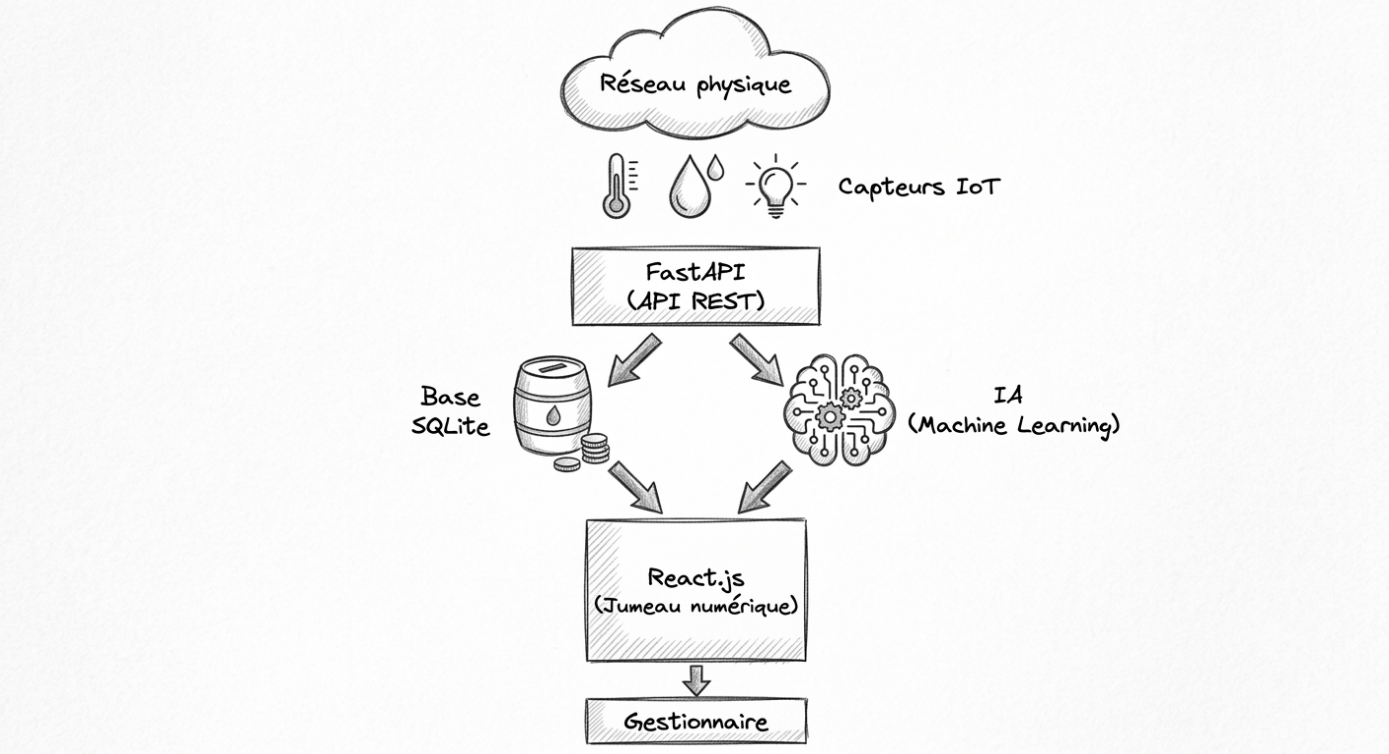
\includegraphics[width=6.3in,height=3.43571in]{figures/image3.png}

Figure 3 Architecture générale du système proposé

\subsection{Architecture physique}

L\textquotesingle architecture physique représente les équipements
matériels intervenant dans le fonctionnement du système.

Elle comprend principalement :

\begin{itemize}
	\item
	les infrastructures hydrauliques (réservoirs, conduites, stations de
	pompage) ;
	\item
	les capteurs intelligents installés sur le réseau ;
	\item
	le serveur hébergeant l\textquotesingle API et la base de données ;
	\item
	les ordinateurs utilisés par les gestionnaires du réseau ;
	\item
	la connexion réseau permettant la communication entre les différents
	composants.
\end{itemize}

Cette architecture permet d'intégrer les données disponibles au
prototype et de les transmettre vers la plateforme numérique pour leur
exploitation \cite{ref20}.

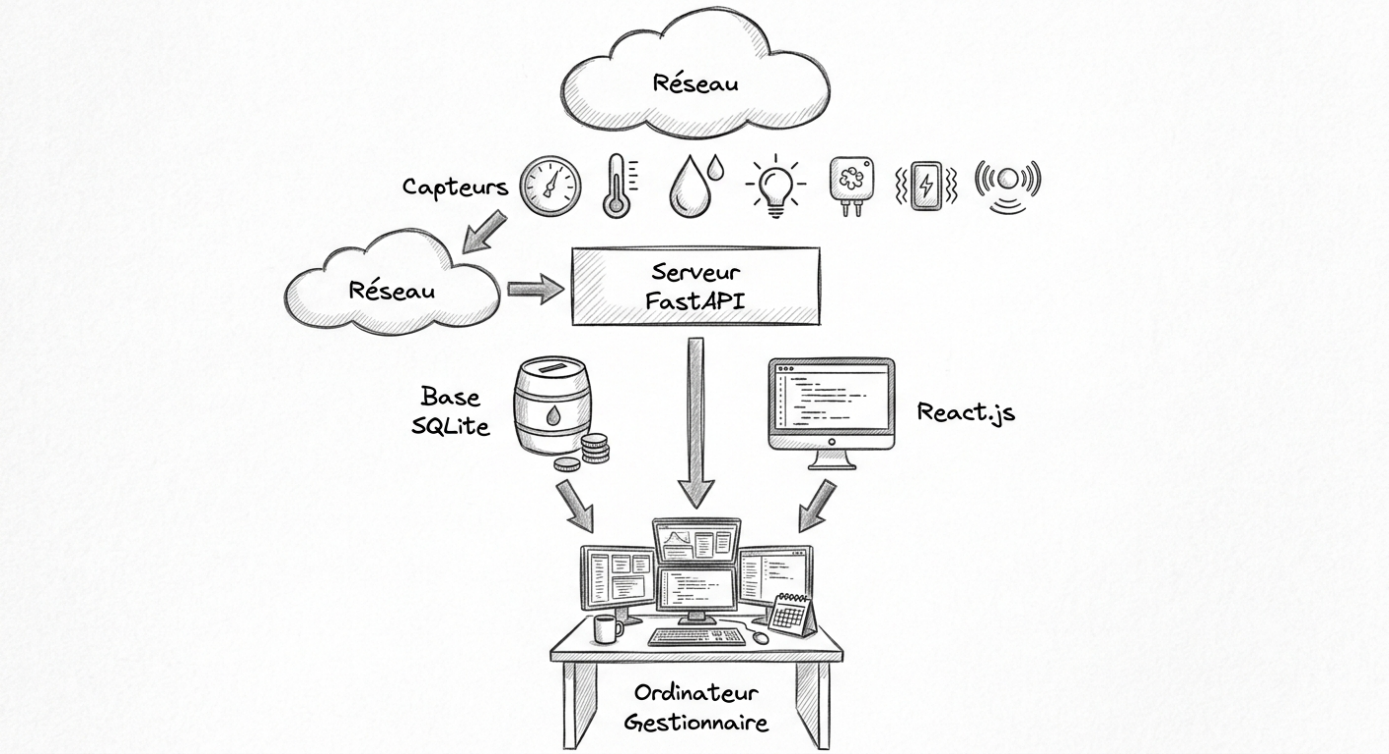
\includegraphics[width=6.3in,height=3.43571in]{figures/image4.png}

Figure 4 Architecture physique

\subsection{Architecture logicielle}\label{architecture-logicielle}

L\textquotesingle application est développée selon une architecture en
couches (\emph{Layered Architecture}), permettant de séparer clairement
les différentes responsabilités.

Elle est composée de :

\subsubsection{Couche de présentation}\label{couche-de-pruxe9sentation}

Développée avec \textbf{React.js (Vite - JSX)}, cette couche permet aux
utilisateurs de visualiser les informations du réseau, les cartes
interactives, les statistiques et les alertes.

\subsubsection{Couche métier}\label{couche-muxe9tier}

Cette couche est développée avec \textbf{FastAPI}. Elle contient toute
la logique métier, notamment :

\begin{itemize}
	\item
	gestion des utilisateurs ;
	\item
	gestion des équipements ;
	\item
	traitement des données ;
	\item
	communication avec l\textquotesingle IA ;
	\item
	génération des alertes.
\end{itemize}

\subsubsection{Couche intelligence
	artificielle}\label{couche-intelligence-artificielle}

Elle réalise :

\begin{itemize}
	\item
	la détection des anomalies ;
	\item
	la prédiction des pannes ;
	\item
	l\textquotesingle analyse des tendances ;
	\item
	les recommandations de maintenance.
\end{itemize}

\subsubsection{Couche données}\label{couche-donnuxe9es}

Cette couche correspond à \textbf{SQLite}, qui stocke :

\begin{itemize}
	\item
	utilisateurs ;
	\item
	capteurs ;
	\item
	équipements ;
	\item
	mesures ;
	\item
	alertes ;
	\item
	historiques.
\end{itemize}

L\textquotesingle utilisation d\textquotesingle une architecture
multicouche améliore la modularité, facilite la maintenance et permet de
faire évoluer indépendamment chaque composant du système \cite{ref106}.

\subsection{Architecture fonctionnelle}\label{architecture-fonctionnelle}

L\textquotesingle architecture fonctionnelle décrit les principaux
traitements réalisés par le système.

Le fonctionnement général est le suivant :

\begin{enumerate}
	\def\labelenumi{\arabic{enumi}.}
	\item
	Les sources de données fournissent les mesures ou valeurs simulées des
	paramètres du réseau.
	\item
	Les données sont transmises au serveur FastAPI à travers les API REST.
	\item
	Les informations sont enregistrées dans la base de données.
	\item
	Le moteur d\textquotesingle intelligence artificielle analyse les
	mesures.
	\item
	Les anomalies sont détectées.
	\item
	Les alertes sont générées.
	\item
	Les résultats sont affichés sur le jumeau numérique.
	\item
	Les gestionnaires du réseau prennent les décisions nécessaires.
\end{enumerate}

Cette organisation facilite la surveillance du réseau et l'analyse des
anomalies \cite{ref17}.

\subsection{Architecture de déploiement}\label{architecture-de-duxe9ploiement}

Le système est conçu selon une architecture client-serveur.

Le serveur héberge :

\begin{itemize}
	\item
	FastAPI ;
	\item
	SQLite ;
	\item
	le modèle d\textquotesingle intelligence artificielle ;
	\item
	les API REST.
\end{itemize}

Les clients utilisent simplement un navigateur Web.

L\textquotesingle interface React.js communique avec FastAPI via
\textbf{Axios}, qui envoie des requêtes HTTP pour récupérer ou
transmettre les données.

Cette architecture permet un déploiement aussi bien sur un serveur local
que sur un serveur cloud sans modification majeure de
l\textquotesingle application \cite{ref114}.

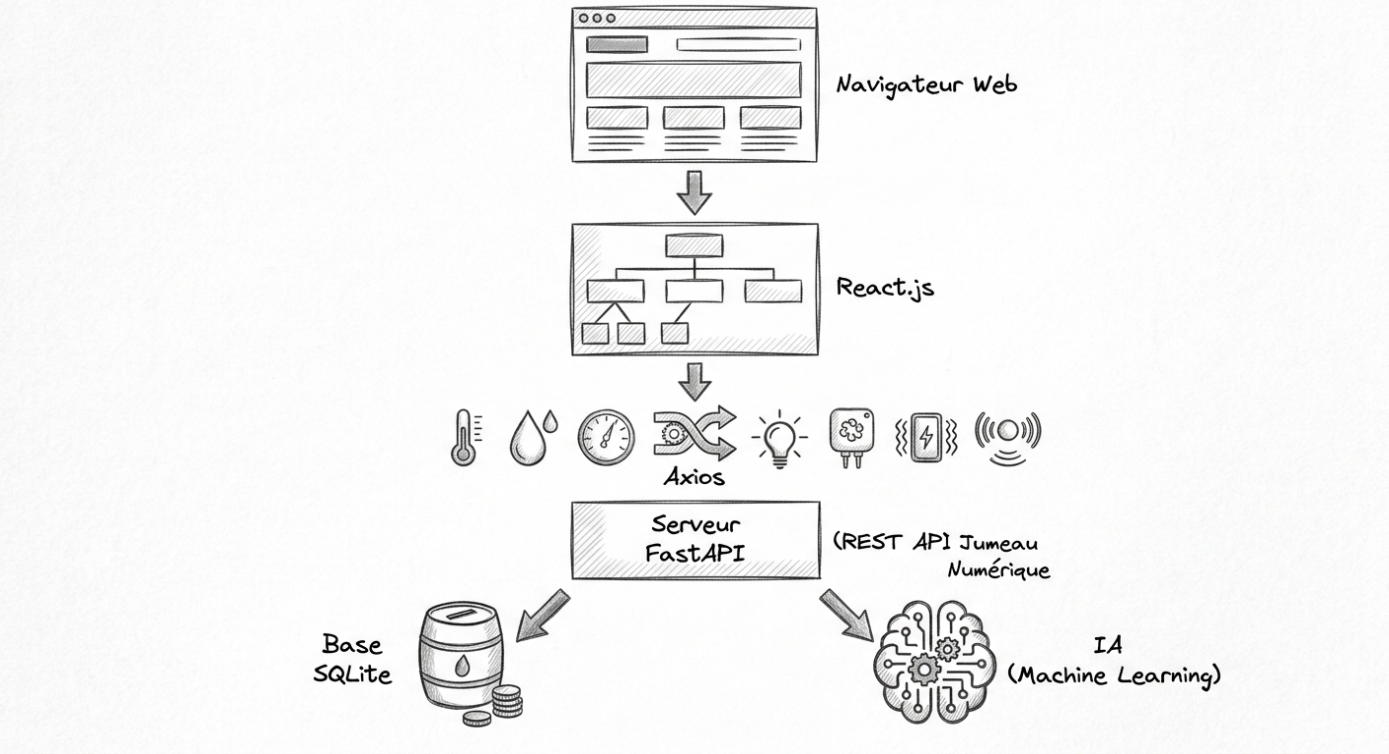
\includegraphics[width=6.3in,height=3.43571in]{figures/image5.png}

Figure 5 Architecture de déploiement

\clearpage
	
	% 4. Bibliographie
	\cleardoublepage
	\printbibliography[heading=bibintoc, title={Références bibliographiques}]
	
\end{document}